\section{Simulation and Results analysis}

In this section are presented the simulations performed on the LNA circuit in the three technologies mentioned before, including the analysis of the gain, noise figure, and input/output impedance. The simulations were conducted using LTSpice and Cadence, and the results are compared with theoretical expectations, and the technologies are compared in terms of performance metrics. 

\subsection{Simulation for 350 nm technology node}

The simulations for this technology were done in LTSpice.
\subsubsection{1:1 $g_m$ ratio}

The results of the s parameters for the 350 nm technology with a 1:1 $g_m$ ratio are shown in Figure \ref{fig:350nm_1to1}. 
\begin{figure}[H]
    \centering
    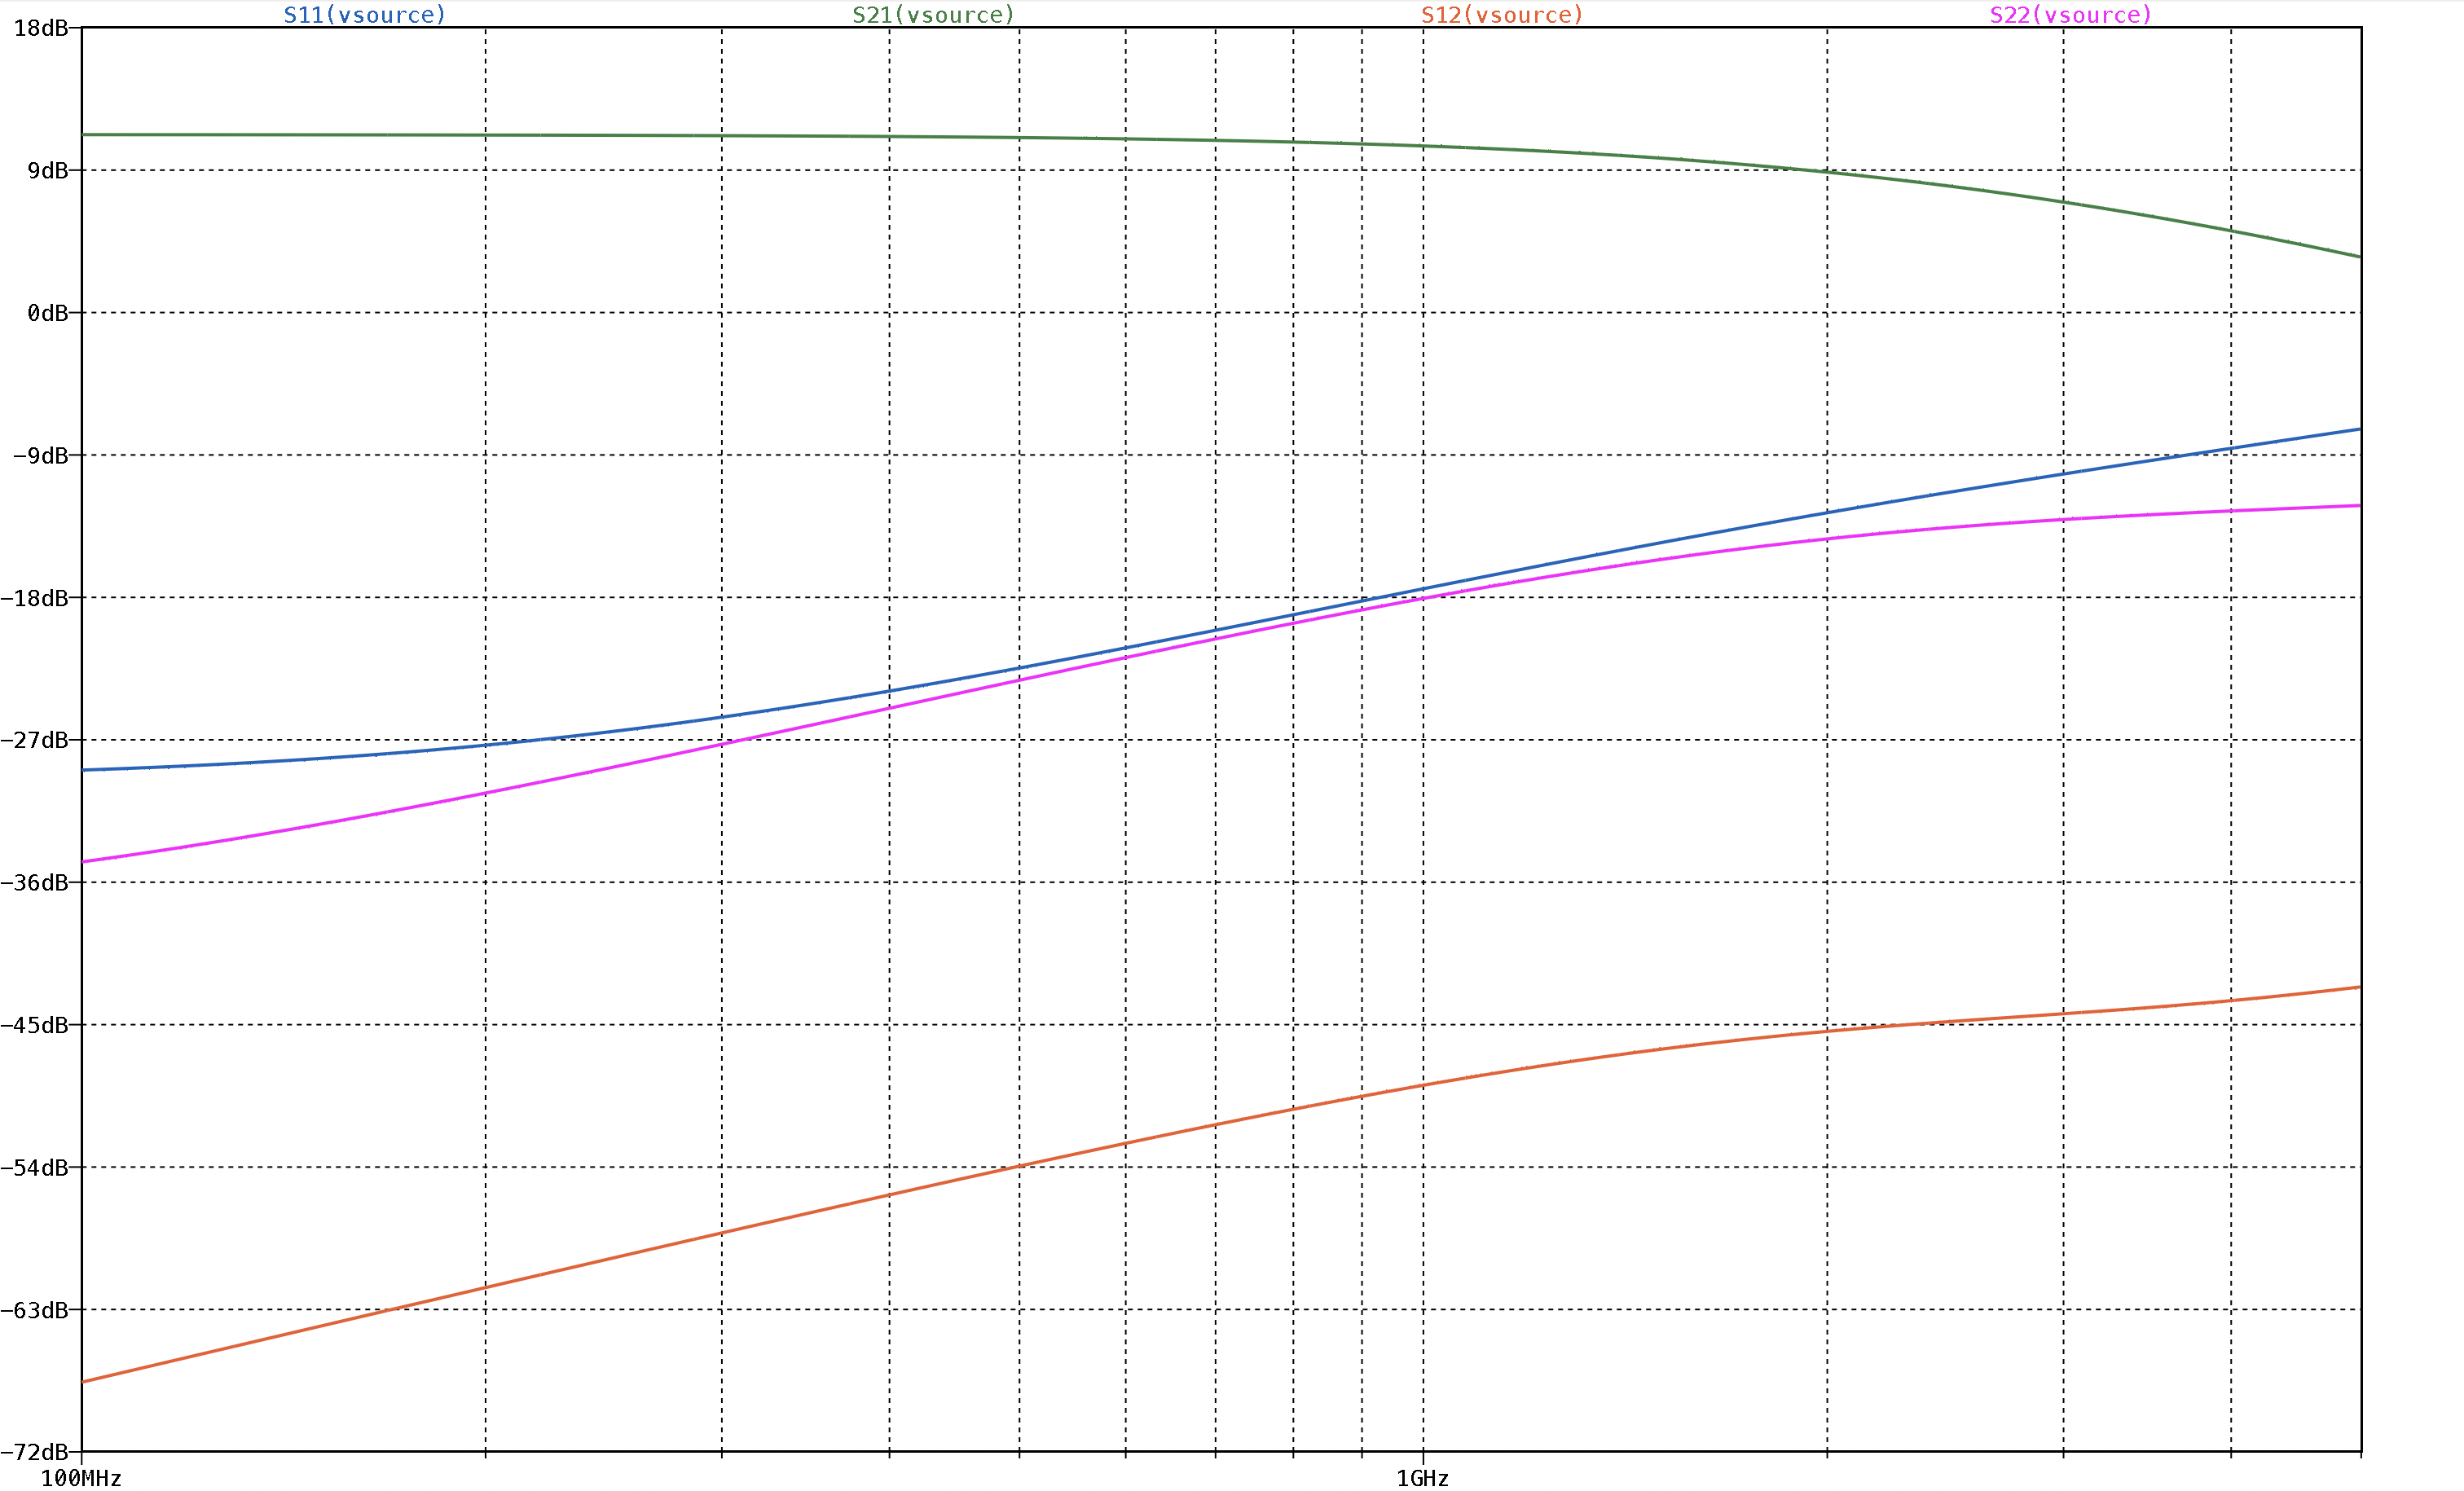
\includegraphics[width=1\textwidth]{Images/3501to1SParam.png}
    \caption{S parameters simulation for 350 nm Technology with 1:1 $g_m$ Ratio}
    \label{fig:350nm_1to1}
\end{figure}

The results for the input and output impedances are shown in Figure \ref{fig:350nm_1to1-Z}.

\begin{figure}[H]
    \centering
    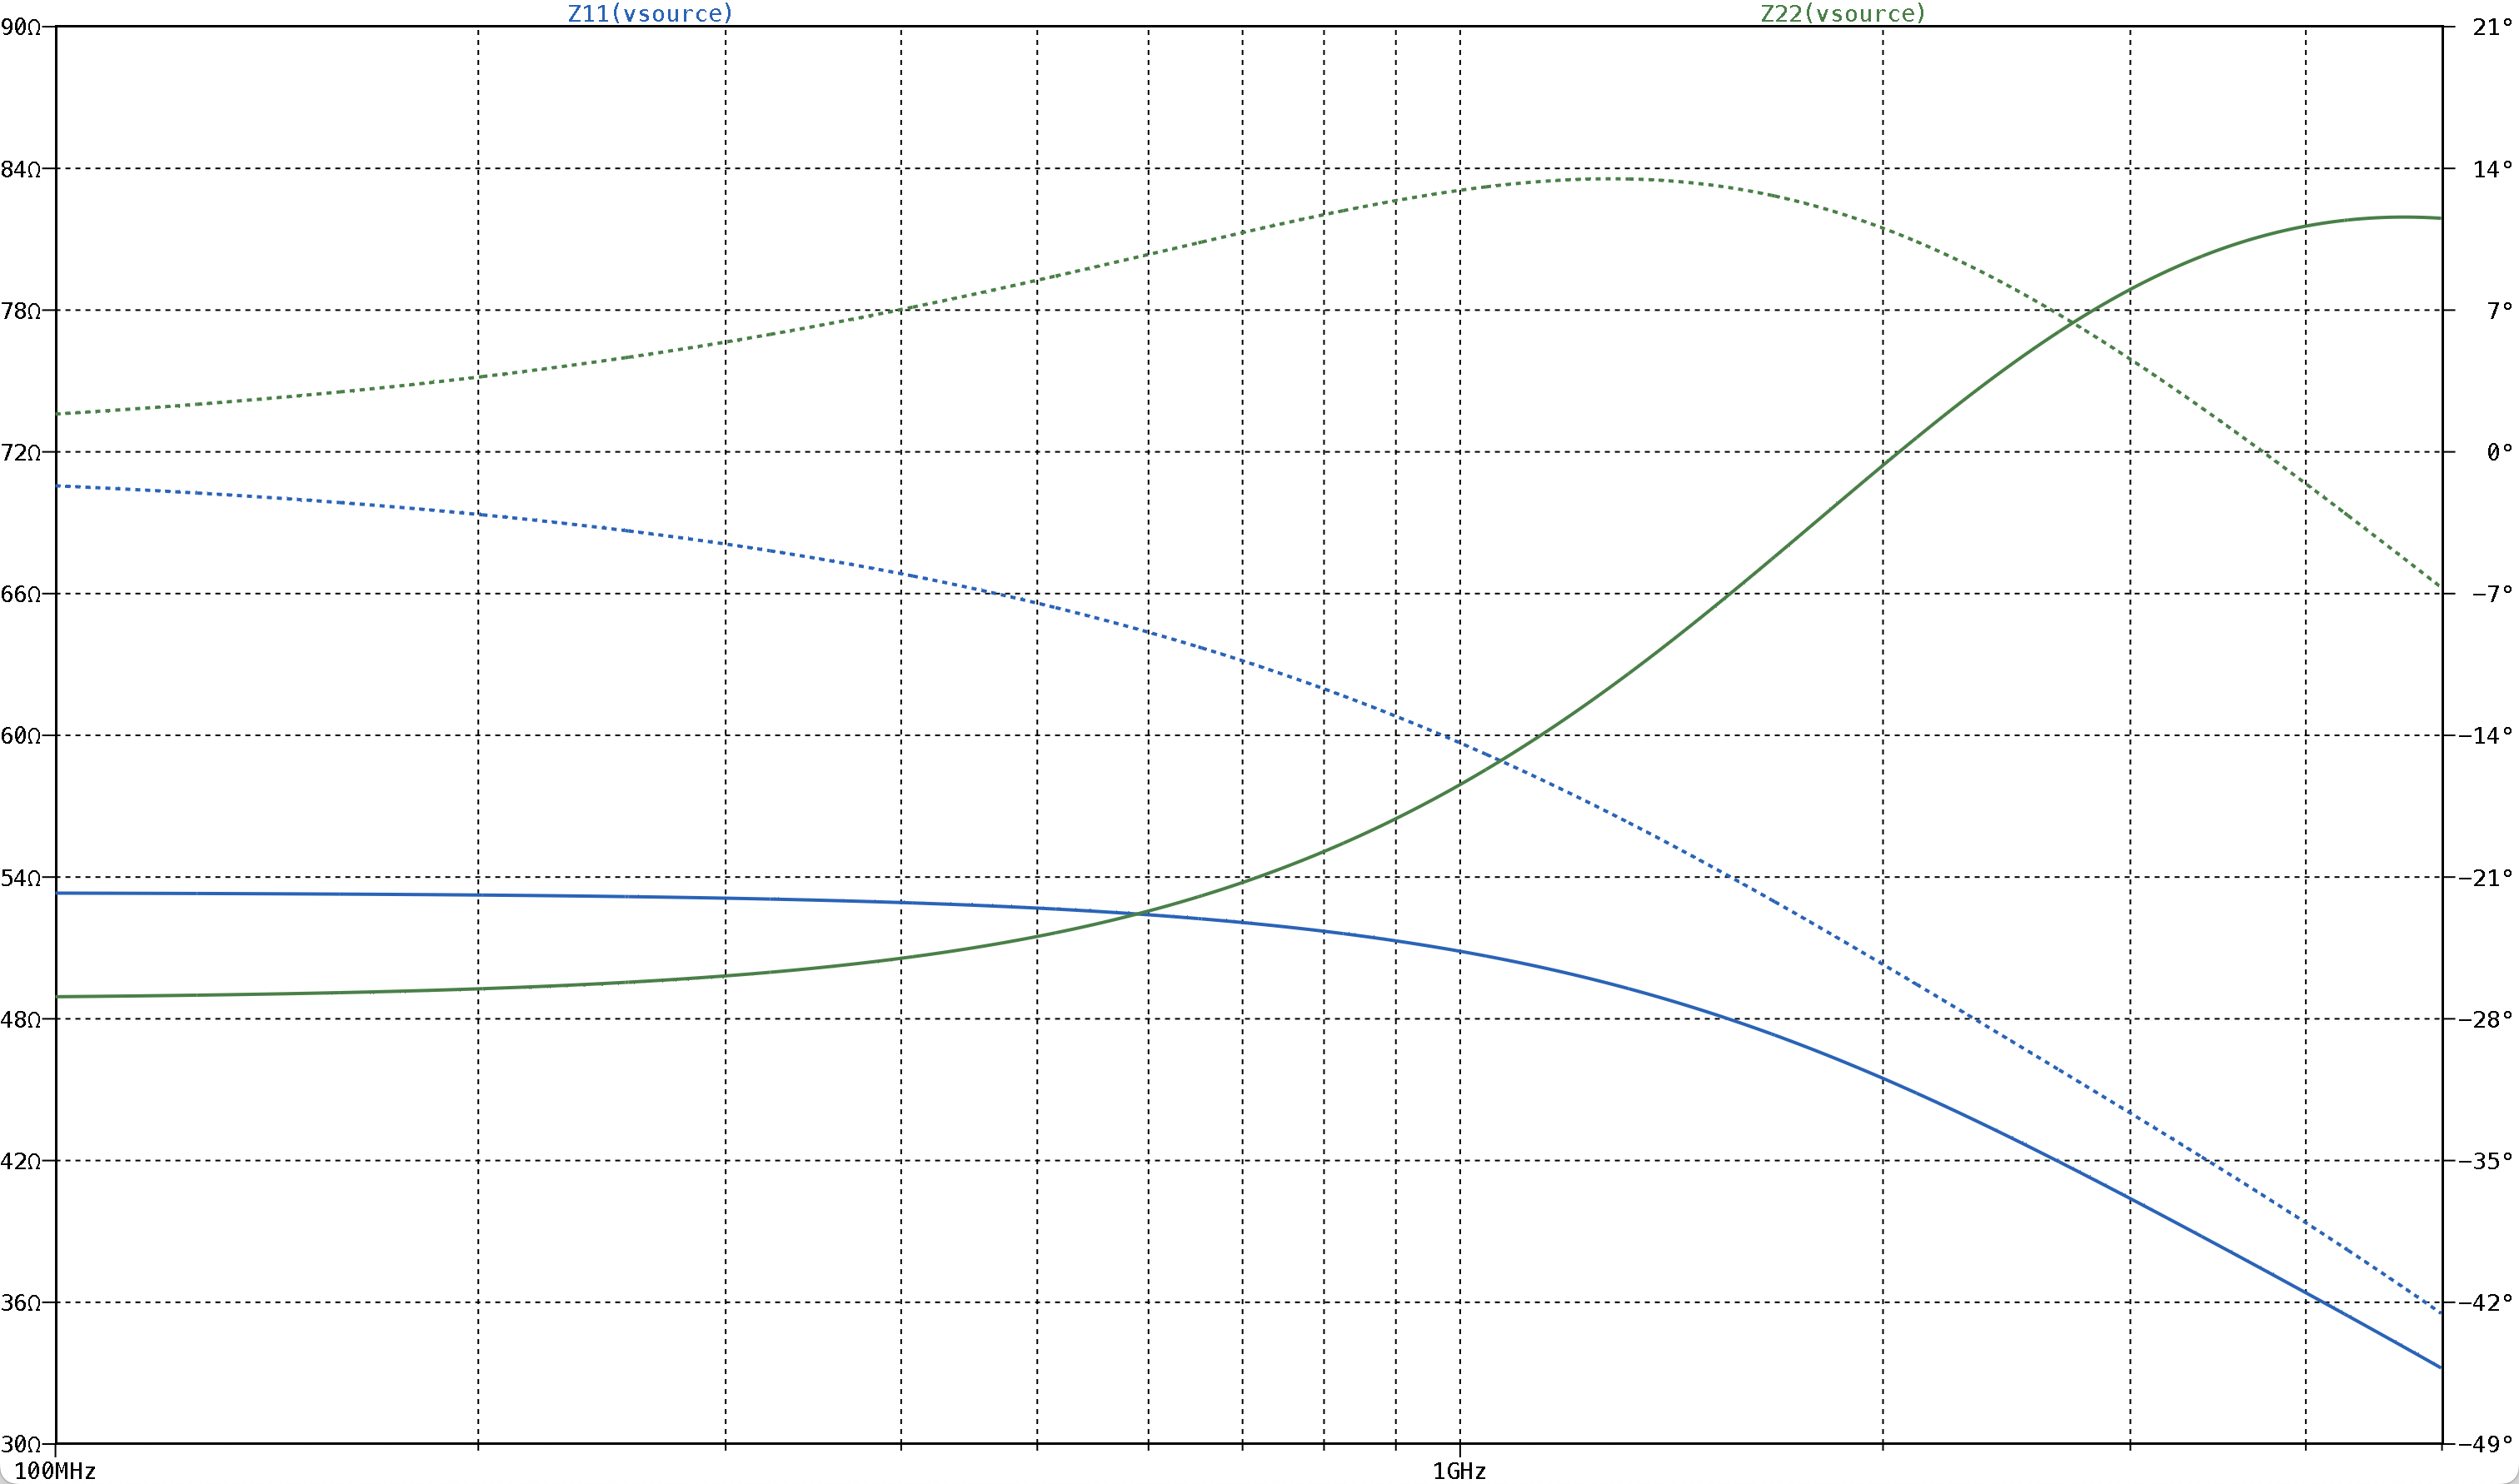
\includegraphics[width=0.9\textwidth]{Images/3501to1ZParam.png}
    \caption{Input and Output Impedances for 350 nm Technology with 1:1 $g_m$ Ratio}
    \label{fig:350nm_1to1-Z}
\end{figure}

Lastly the simulation of the noise factor is shown in Figure \ref{fig:350nm_1to1-NF}.
\begin{figure}[H]
    \centering
    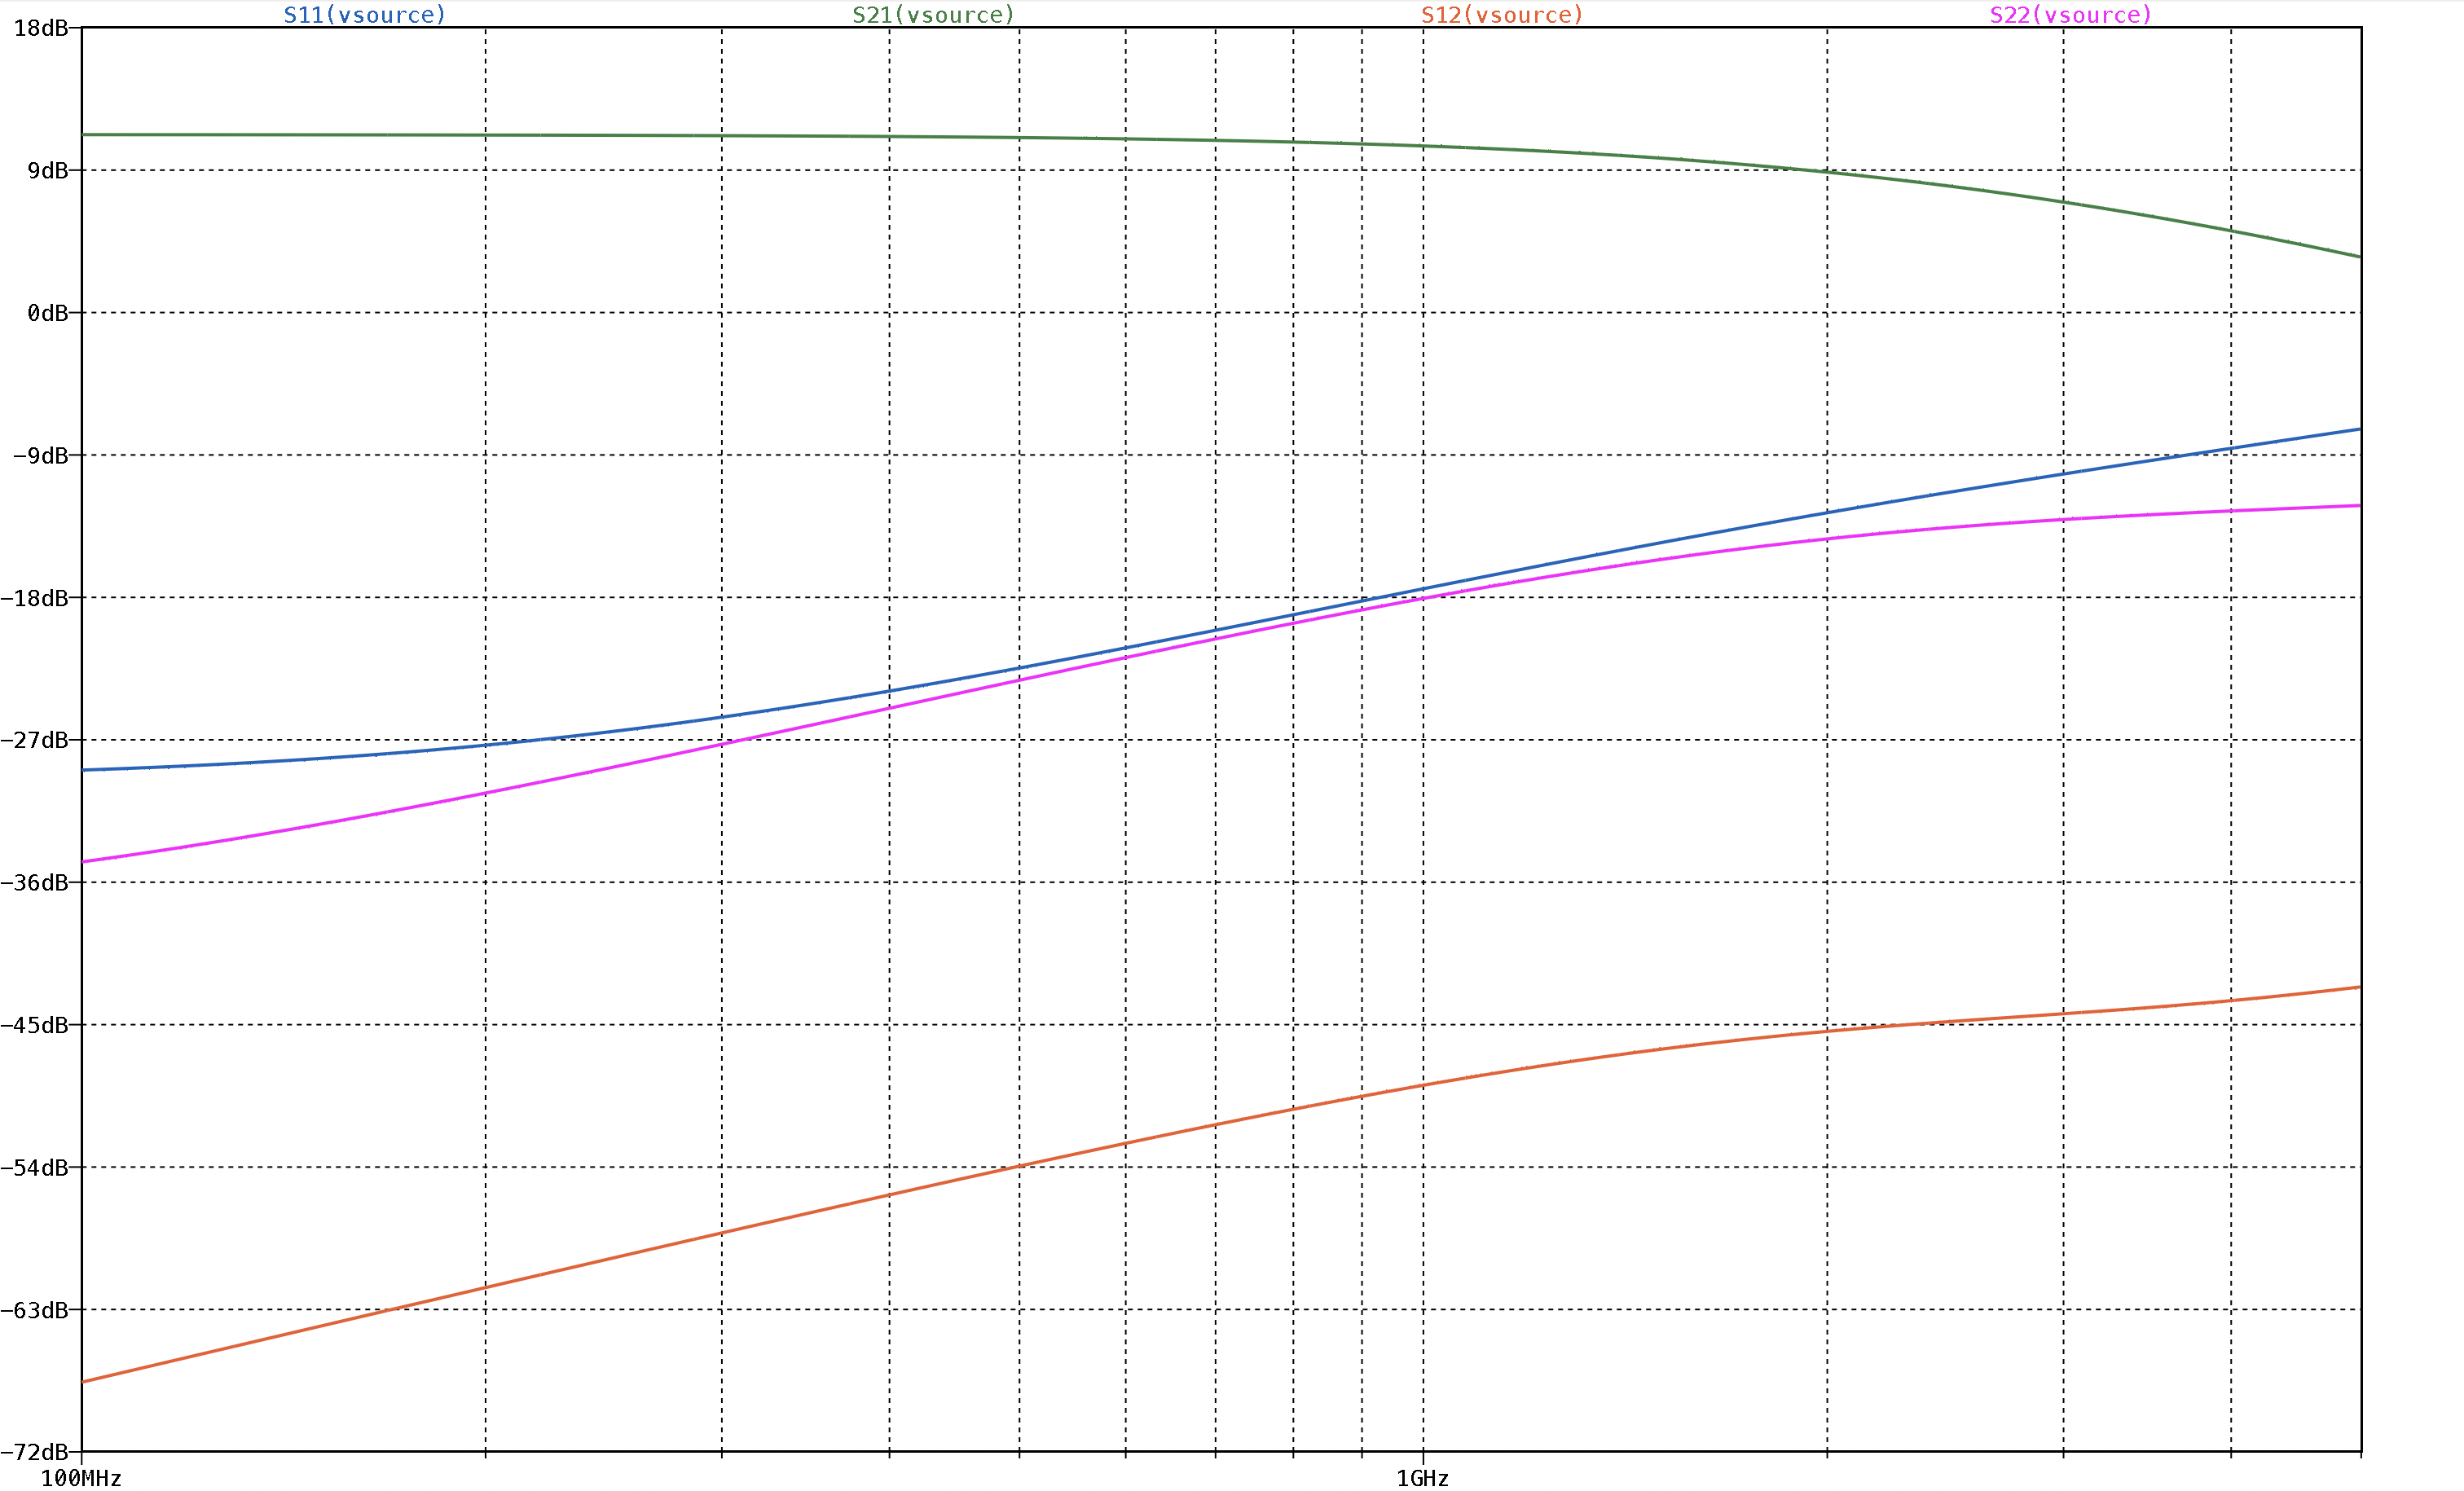
\includegraphics[width=0.9\textwidth]{Images/3501to1SParam.png}
    \caption{Noise Figure for 350 nm Technology with 1:1 $g_m$ Ratio}
    \label{fig:350nm_1to1-NF}
\end{figure}

\begin{table}[H]
    \centering
    \caption{Simulation Results for 350 nm Technology with 1:1 $g_m$ Ratio}
    \begin{tabularx}{\textwidth}{>{\centering\arraybackslash}X >{\centering\arraybackslash}X }
        \toprule
        \textbf{Parameter} & \textbf{Value}\\
        \midrule
        Gain (S21) & \SI{10.52}{\decibel} \\
        \midrule
        Noise Figure (NF) & \SI{3.19}{\decibel} \\
        \midrule
        Input Impedance (Z11) & \SI{50.84}{\ohm} \\
        \midrule
        Output Impedance (Z22) & \SI{57.94}{\ohm} \\
        \midrule
        Frequency & \SI{1}{\giga \hertz} \\
        \bottomrule
    \end{tabularx}
    \label{tab:350nm_1to1_results}
\end{table}
\subsubsection{1:3 $g_m$ ratio}

The results of the s parameters for the 350 nm technology with a 1:3 $g_m$ ratio are shown in Figure \ref{fig:350nm_1ton}. 
\begin{figure}[H]
    \centering
    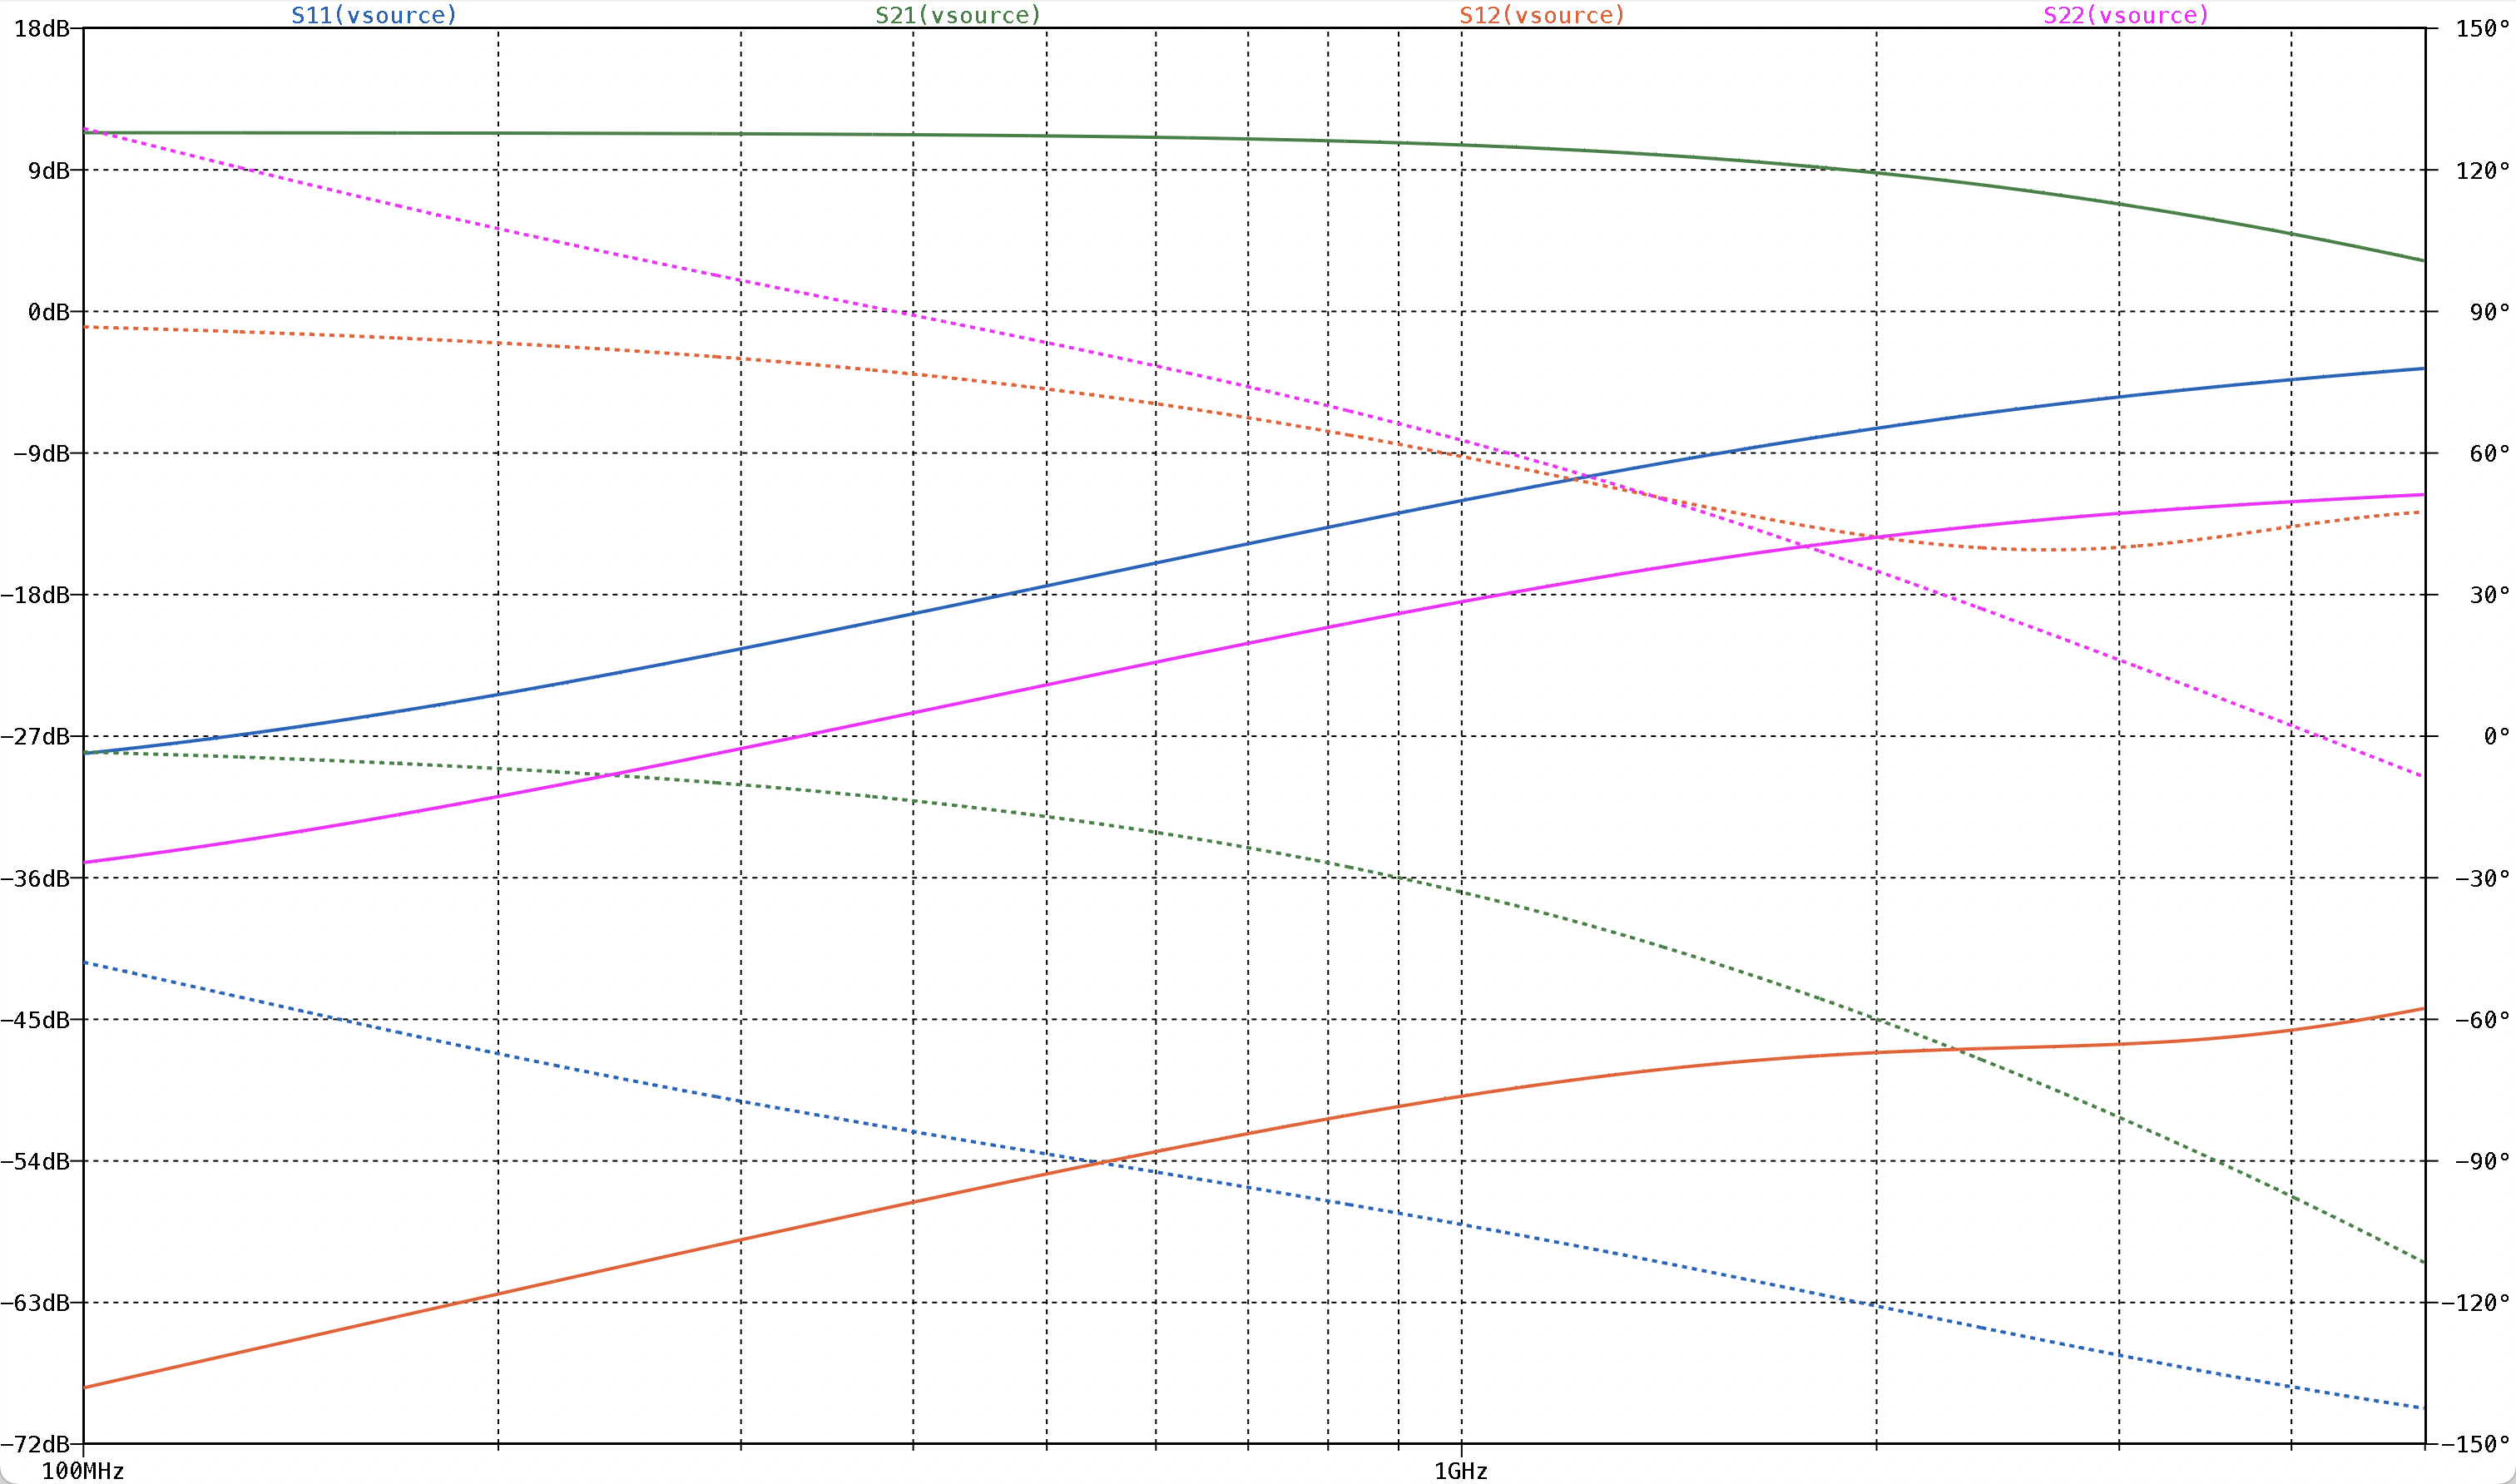
\includegraphics[width=1\textwidth]{Images/3501to3SParam.png}
    \caption{S parameters simulation for 350 nm Technology with 1:3 $g_m$ Ratio}
    \label{fig:350nm_1ton}
\end{figure}

The results for the input and output impedances are shown in Figure \ref{fig:350nm_1to1-Z}.

\begin{figure}[H]
    \centering
    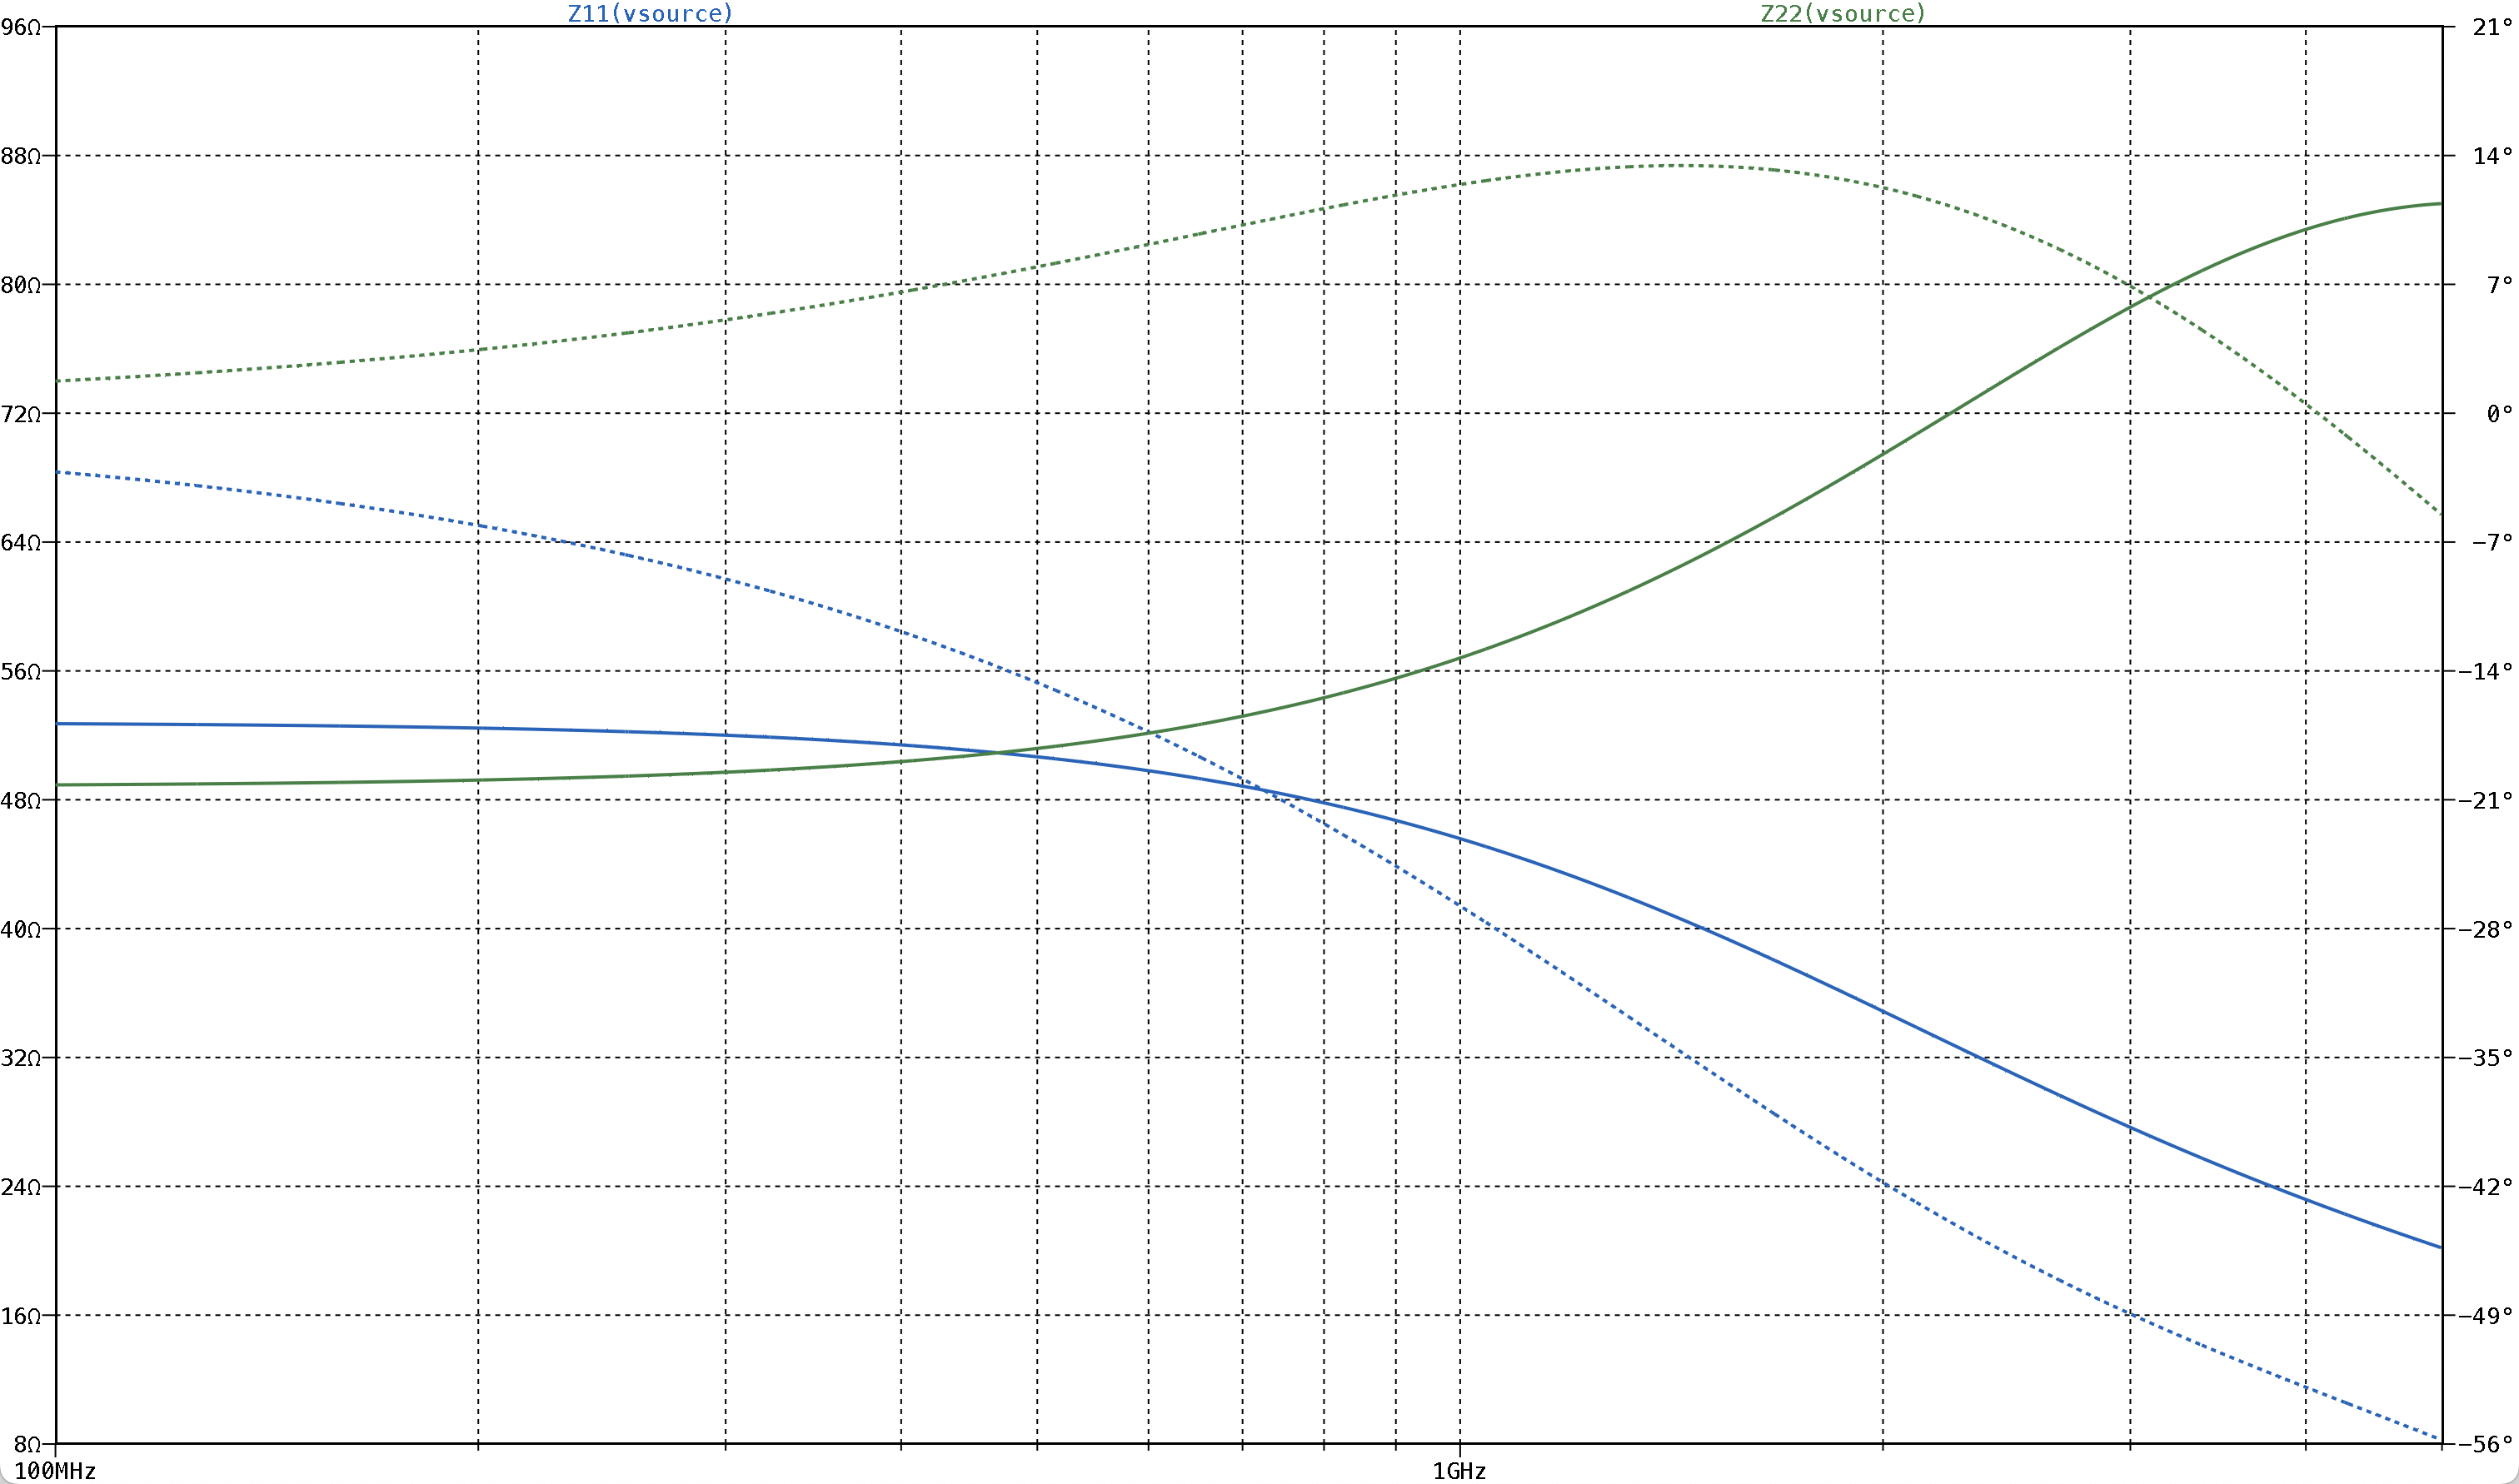
\includegraphics[width=1\textwidth]{Images/3501to3ZParam.png}
    \caption{Input and Output Impedances for 350 nm Technology with 1:3 $g_m$ Ratio}
    \label{fig:350nm_1ton-Z}
\end{figure}

Lastly the simulation of the noise factor is shown in Figure \ref{fig:350nm_1ton-NF}.
\begin{figure}[H]
    \centering
    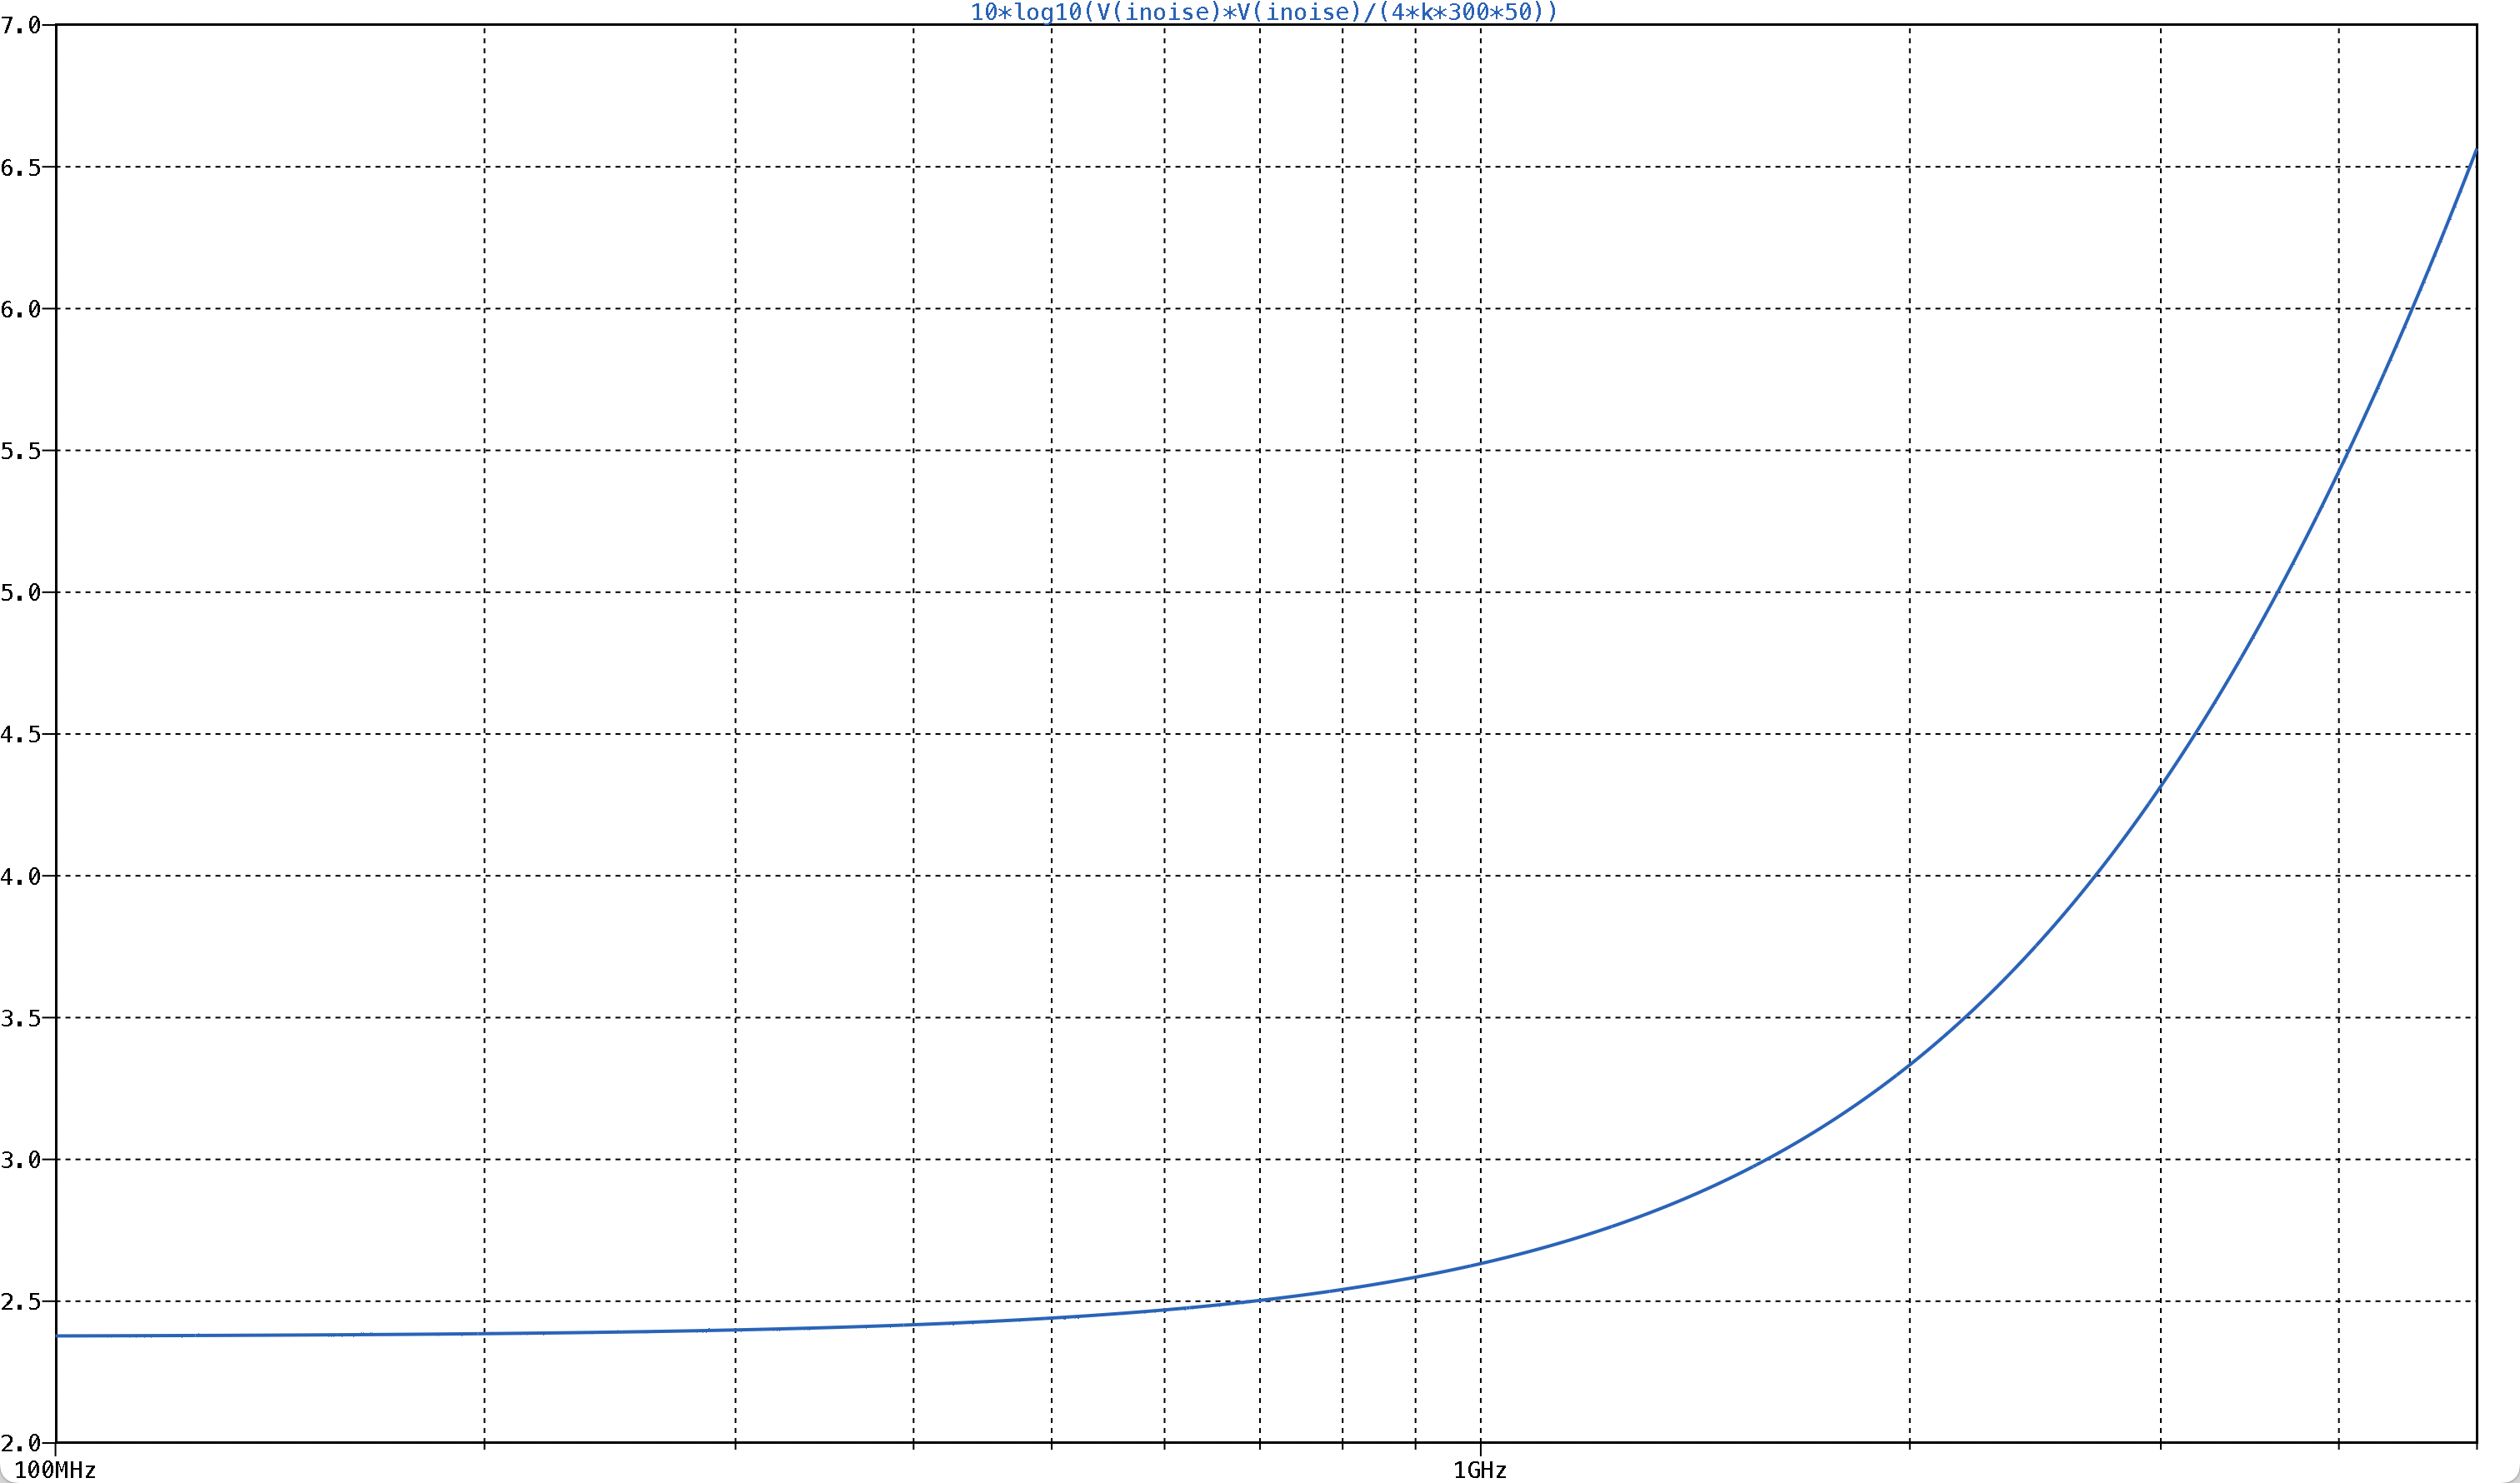
\includegraphics[width=1\textwidth]{Images/3501to3Noise.png}
    \caption{Noise Figure for 350 nm Technology with 1:3 $g_m$ Ratio}
    \label{fig:350nm_1ton-NF}
\end{figure}

\begin{table}[H]
    \centering
    \caption{Simulation Results for 350 nm Technology with 1:3 $g_m$ Ratio}
    \begin{tabularx}{\textwidth}{>{\centering\arraybackslash}X >{\centering\arraybackslash}X }
        \toprule
        \textbf{Parameter} & \textbf{Value}\\
        \midrule
        Gain (S21) & \SI{10.58}{\decibel} \\
        \midrule
        Noise Figure (NF) & \SI{2.64}{\decibel} \\
        \midrule
        Input Impedance (Z11) & \SI{45.58}{\ohm} \\
        \midrule
        Output Impedance (Z22) & \SI{56.82}{\ohm} \\
        \midrule
        Frequency & \SI{1}{\giga \hertz} \\
        \bottomrule
    \end{tabularx}
    \label{tab:350nm_1ton_results}
\end{table}

\subsection{Simulation for 65 nm Technology Node}

The simulations for this technology were done in Cadence. 

\subsubsection{1:1 $g_m$ ratio}

The circuit implemented in Cadence for the 65 nm technology with a 1:1 $g_m$ ratio is shown in Figure \ref{fig:65nm_1to1-circ}. The simulation results are shown in Figure \ref{fig:65nm_1to1} summarized in Table \ref{tab:65nm_1to1_results}.
\begin{figure}[H]
    \centering
    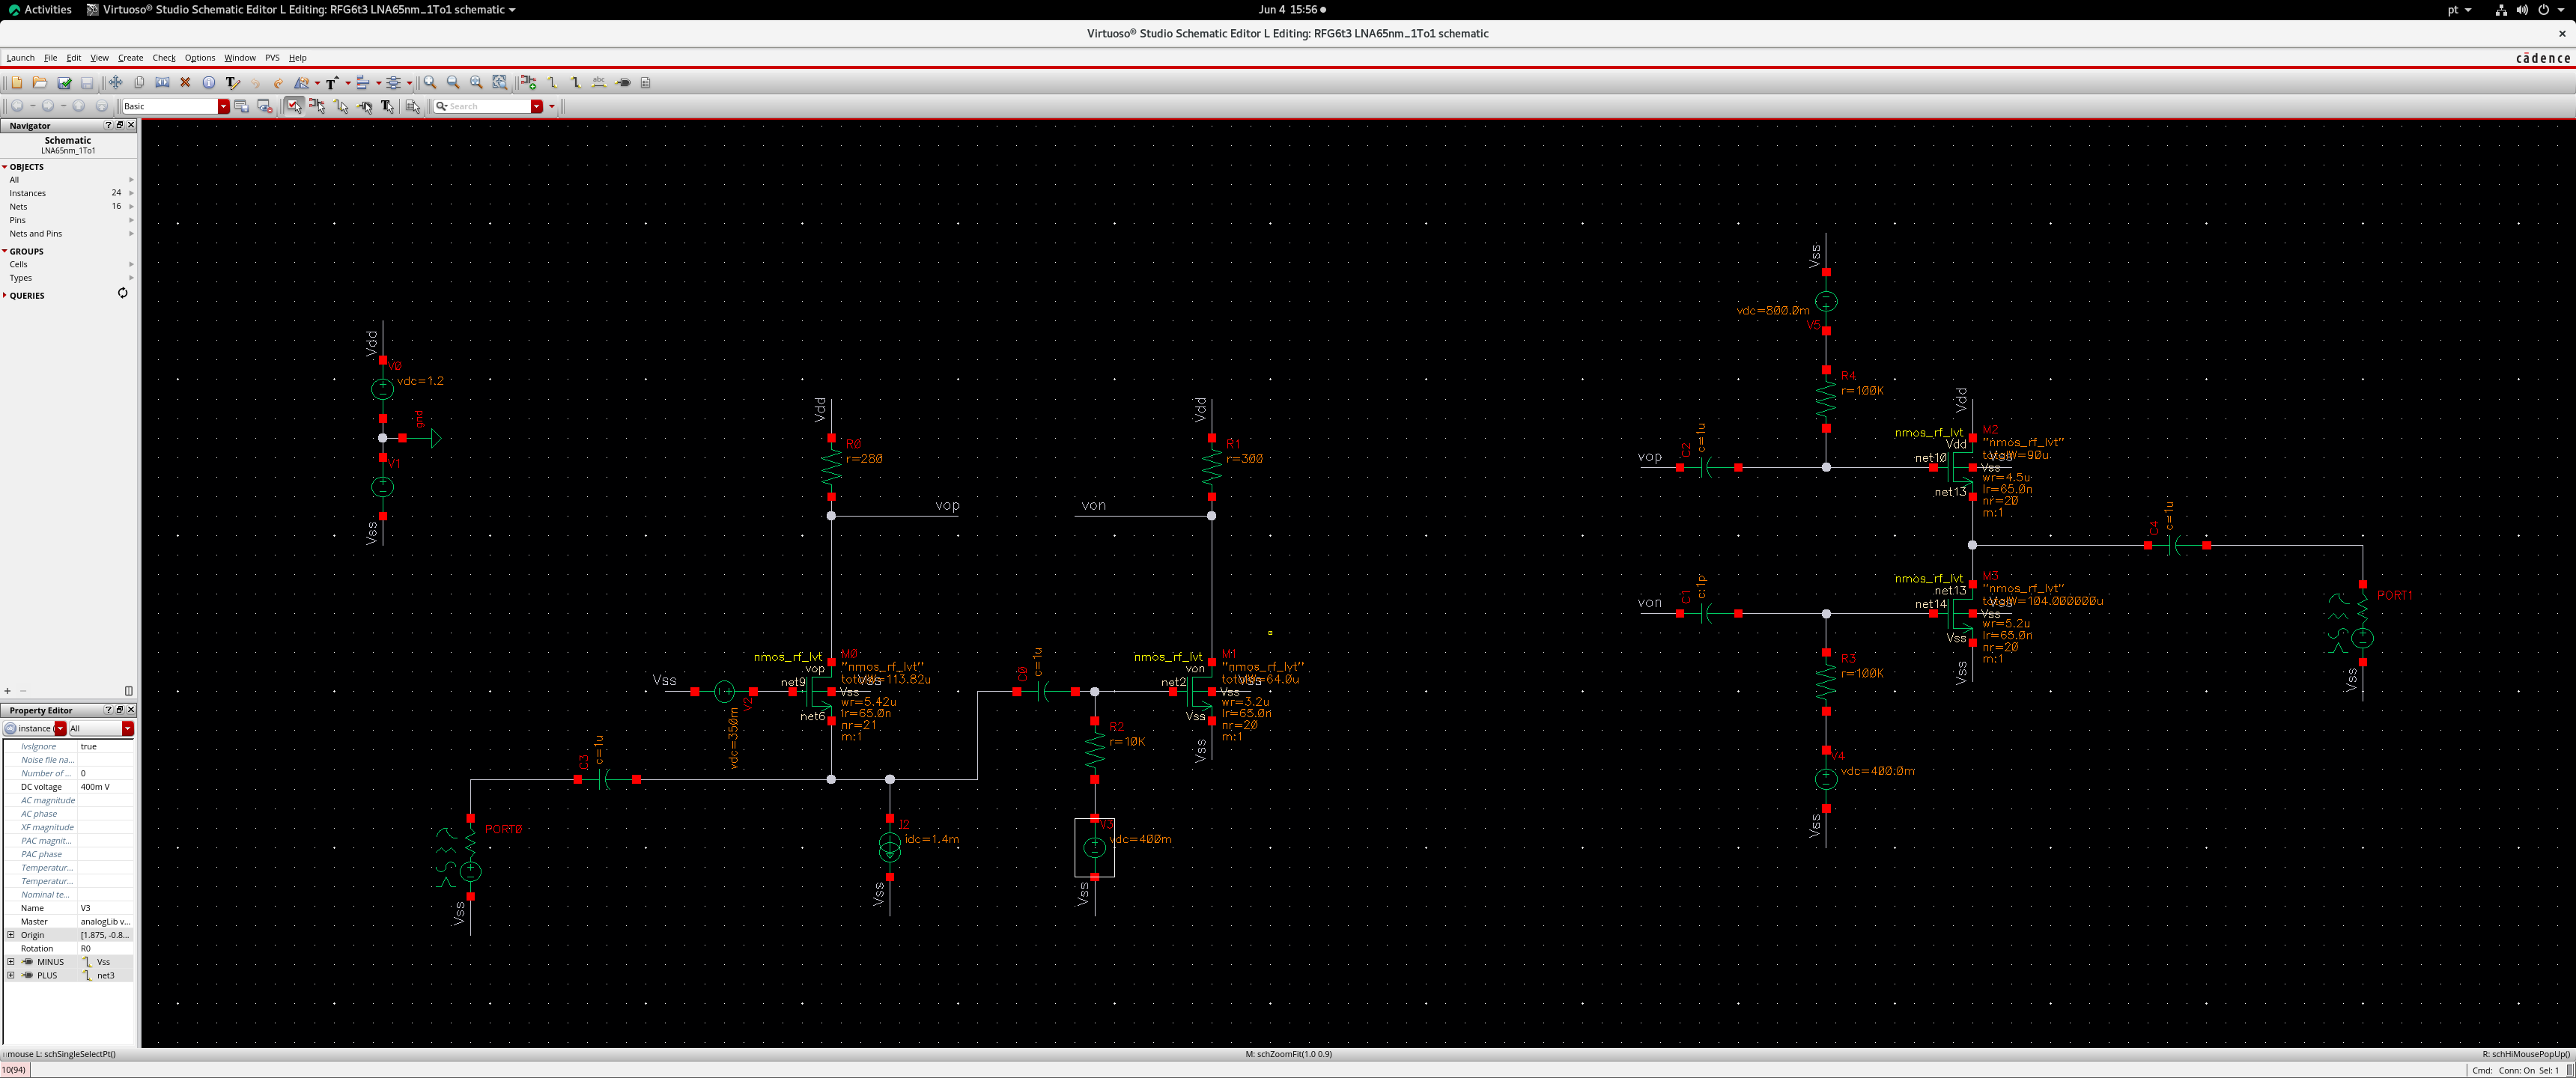
\includegraphics[width=1\textwidth]{Images/65nm1To1Circ.png}
    \caption{LNA Circuit for 65 nm Technology with 1:1 $g_m$ Ratio}
    \label{fig:65nm_1to1-circ}
\end{figure}

\begin{figure}[H]
    \centering
    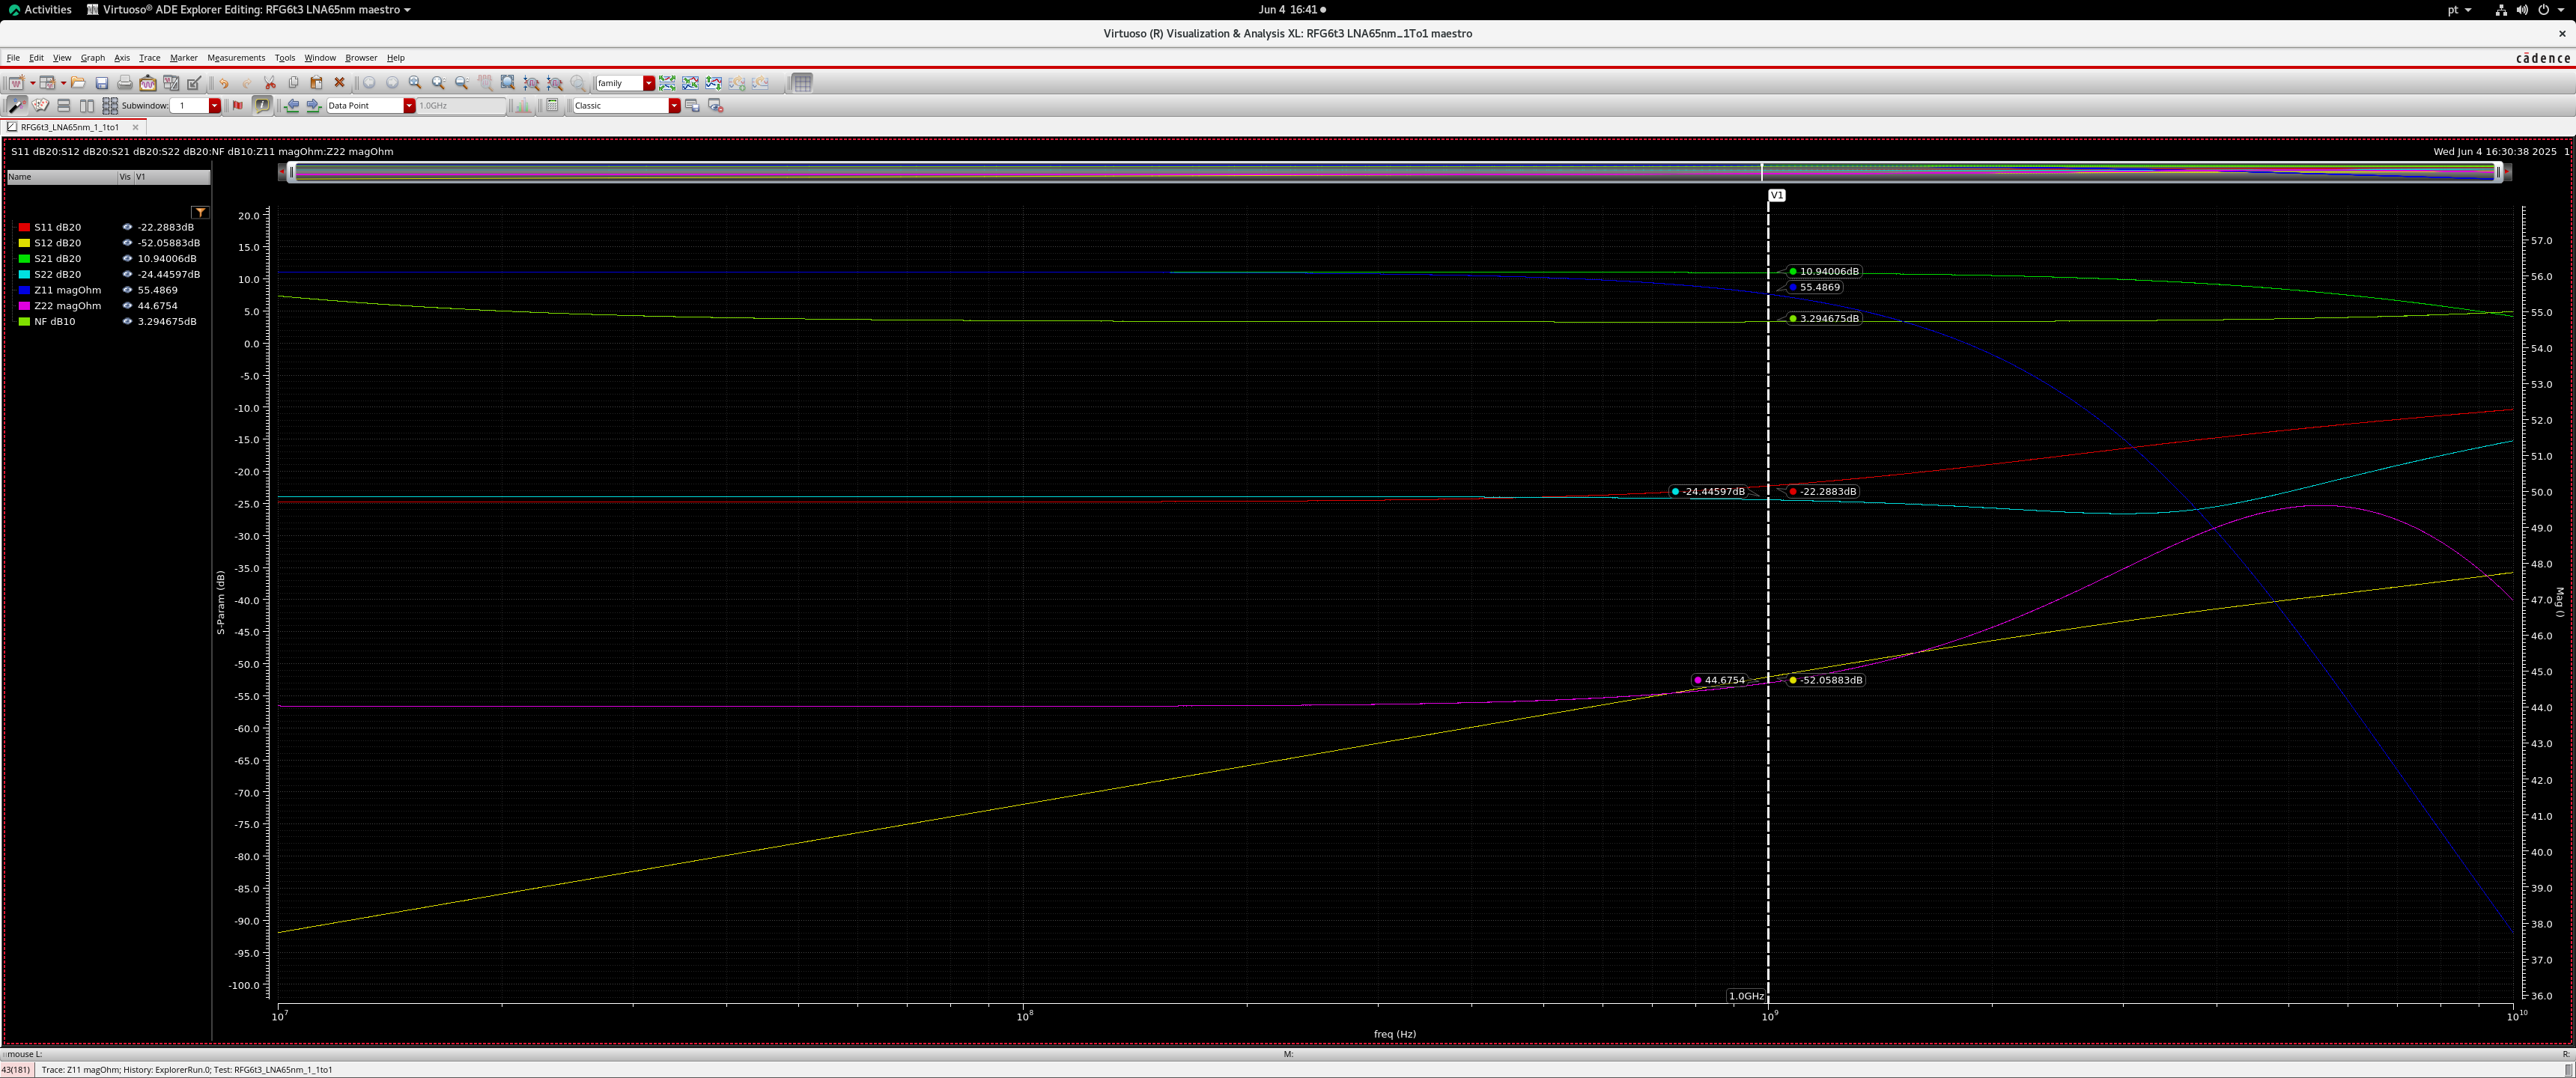
\includegraphics[width=1\textwidth]{Images/65nm1to1.png}
    \caption{LNA Simulation for 65 nm Technology with 1:1 $g_m$ Ratio}
    \label{fig:65nm_1to1}
\end{figure}

\begin{table}[H]
    \centering
    \caption{Simulation Results for 65 nm Technology with 1:1 $g_m$ Ratio}
    \begin{tabularx}{\textwidth}{>{\centering\arraybackslash}X >{\centering\arraybackslash}X }
        \toprule
        \textbf{Parameter} & \textbf{Value}\\
        \midrule
        Gain (S21) & \SI{10.94}{\decibel} \\
        \midrule
        Noise Figure (NF) & \SI{3.29}{\decibel} \\
        \midrule
        Input Impedance (Z11) & \SI{44.68}{\ohm} \\
        \midrule
        Output Impedance (Z22) & \SI{55.49}{\ohm} \\
        \midrule
        Frequency & \SI{5}{\giga \hertz}\\
        \bottomrule
    \end{tabularx}
    \label{tab:65nm_1to1_results}
\end{table}


\subsubsection{1:3 $g_m$ ratio}

The circuit implemented in Cadence for the 65 nm technology with a 1:3 $g_m$ ratio is shown in Figure \ref{fig:65nm_1ton-circ}. The simulation results are shown in Figure \ref{fig:65nm_1ton} summarized in Table \ref{tab:65nm_1ton_results}.

\begin{figure}[H]
    \centering
    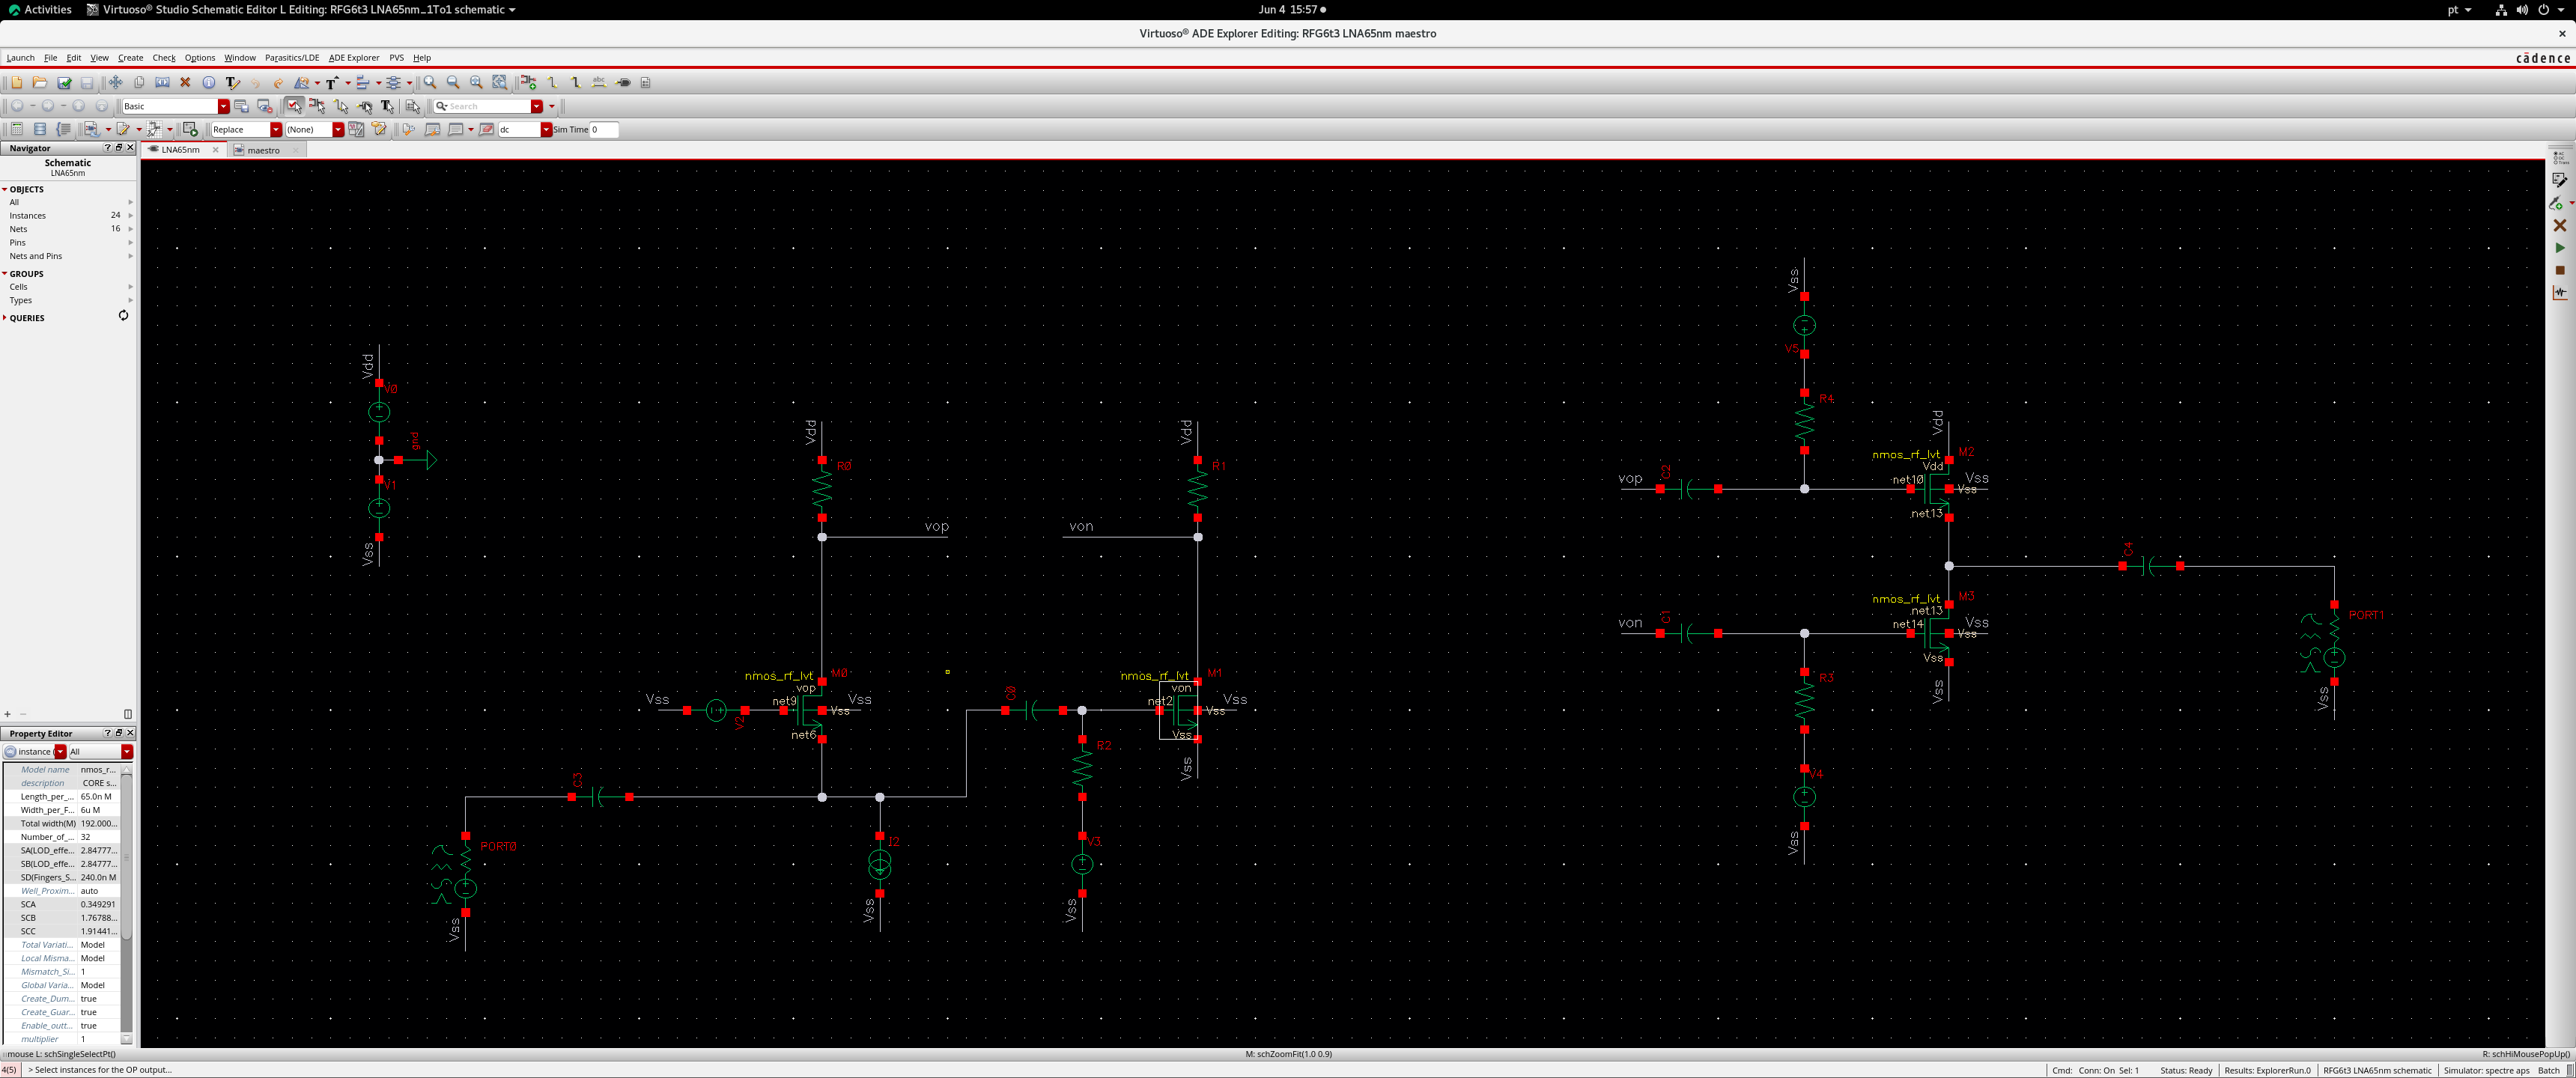
\includegraphics[width=1\textwidth]{Images/65nm1To35Circ.png}
    \caption{LNA Circuit for 65 nm Technology with 1:n $g_m$ Ratio}
    \label{fig:65nm_1ton-circ}
\end{figure}

\begin{figure}[H]
    \centering
    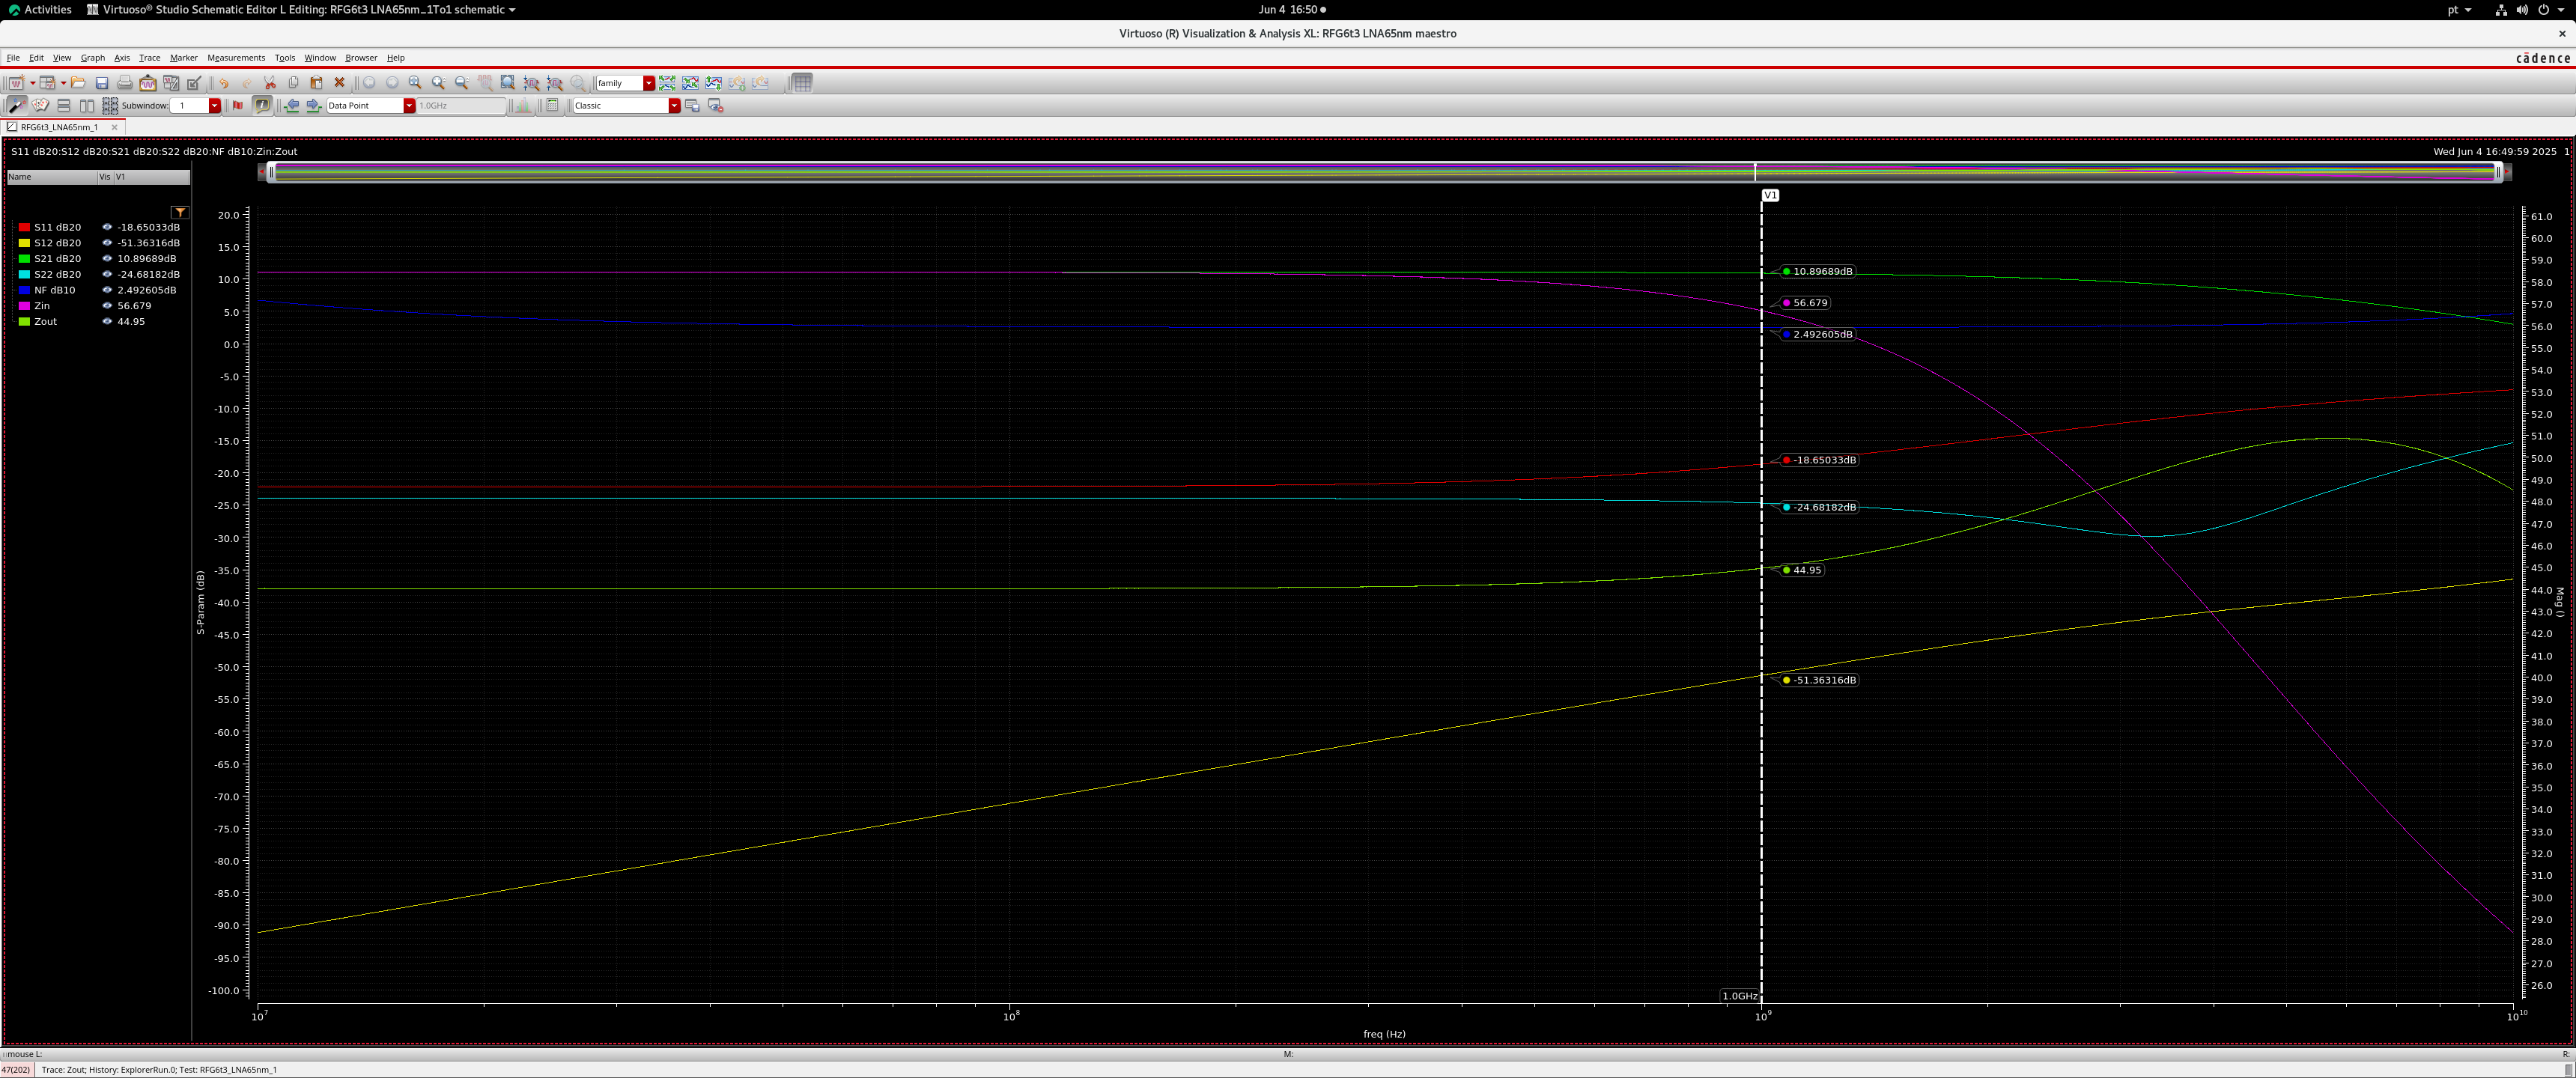
\includegraphics[width=1\textwidth]{Images/65nm1To35Final.png}
    \caption{LNA Simulation for 65 nm Technology with 1:n $g_m$ Ratio}
    \label{fig:65nm_1ton}
\end{figure}

\begin{table}[H]
    \centering
    \caption{Simulation Results for 65 nm Technology with 1:n $g_m$ Ratio}
    \begin{tabularx}{\textwidth}{>{\centering\arraybackslash}X >{\centering\arraybackslash}X }
        \toprule
        \textbf{Parameter} & \textbf{Value}\\
        \midrule
        Gain (S21) & \SI{10.86}{\decibel} \\
        \midrule
        Noise Figure (NF) & \SI{2.49}{\decibel} \\
        \midrule
        Input Impedance (Z11) & \SI{56.68}{\ohm} \\
        \midrule
        Output Impedance (Z22) & \SI{44.95}{\ohm} \\
        \midrule
        Frequency & \SI{5}{\giga \hertz} \\
        \bottomrule
    \end{tabularx}
    \label{tab:65nm_1ton_results}
\end{table}

\subsection{Simulation for 45 nm Technology}

The simulations for this technology were done in LTSpice.
\subsubsection{1:1 $g_m$ ratio}

The results of the s parameters for the 45 nm technology with a 1:1 $g_m$ ratio are shown in Figure \ref{fig:SParam45nm1to1}. 
\begin{figure}[H]
    \centering
    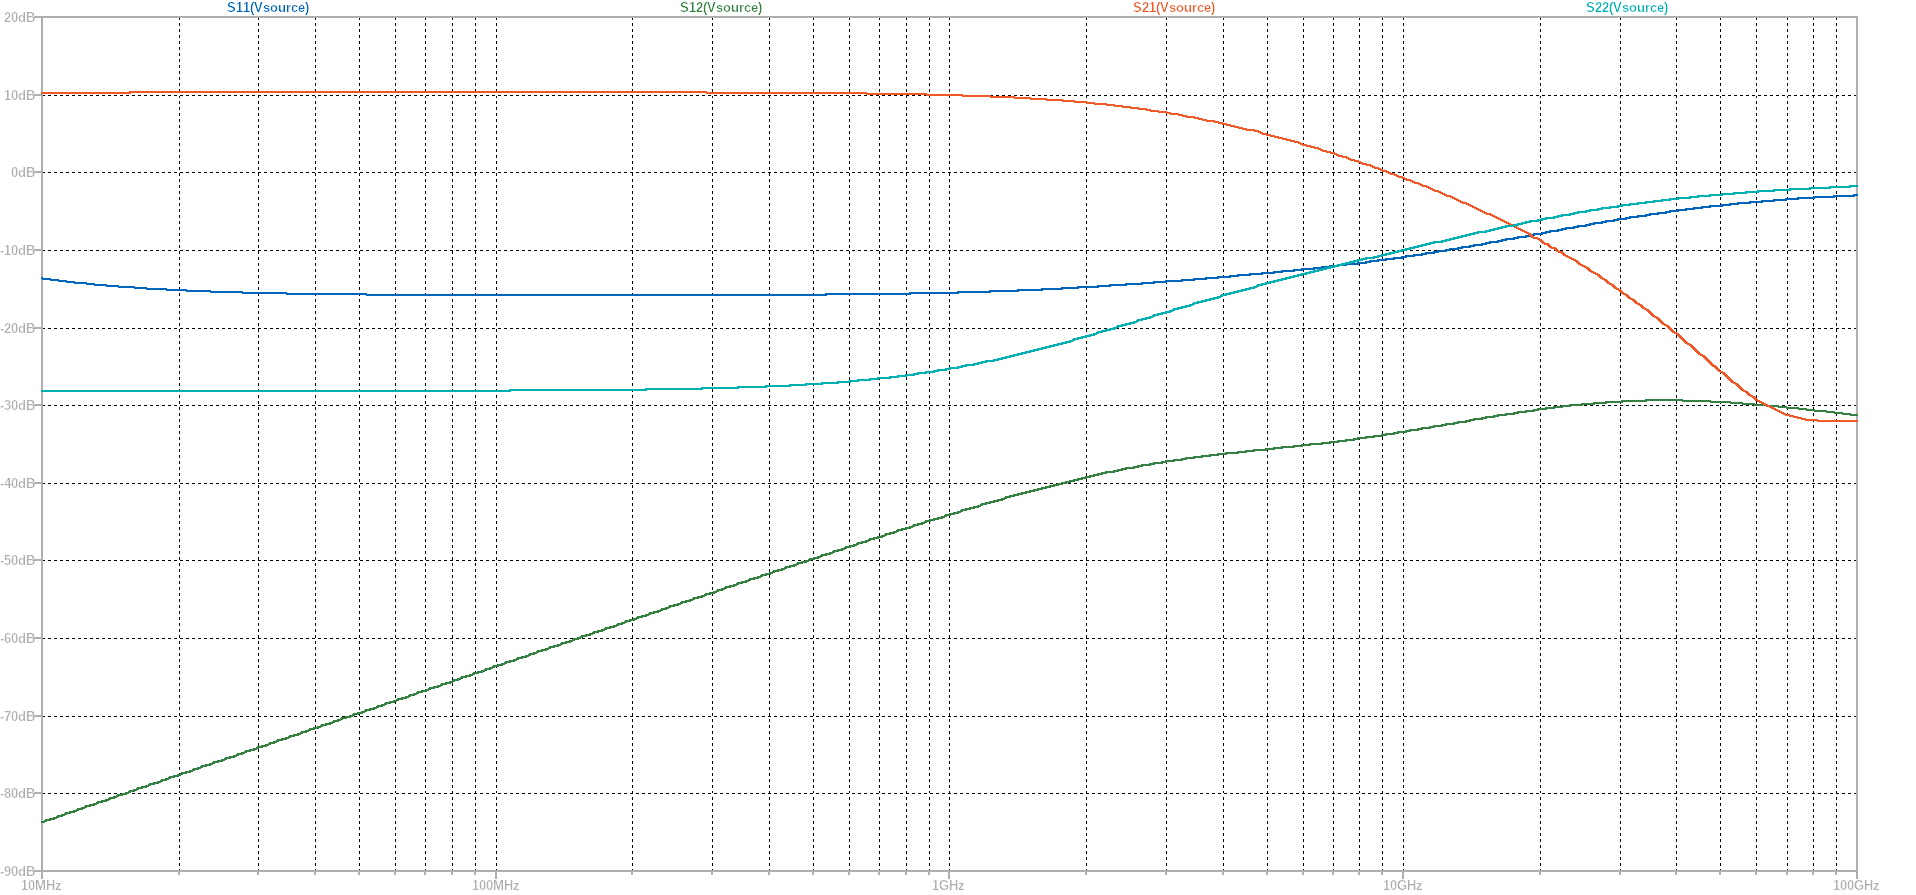
\includegraphics[width=1\textwidth]{Images/SParam_45_1To1.png}
    \caption{S parameters simulation for 45 nm Technology with 1:1 $g_m$ Ratio}
    \label{fig:SParam45nm1to1}
\end{figure}

The results for the input and output impedances are shown in Figure \ref{fig:ZParam45nm1to1}.

\begin{figure}[H]
    \centering
    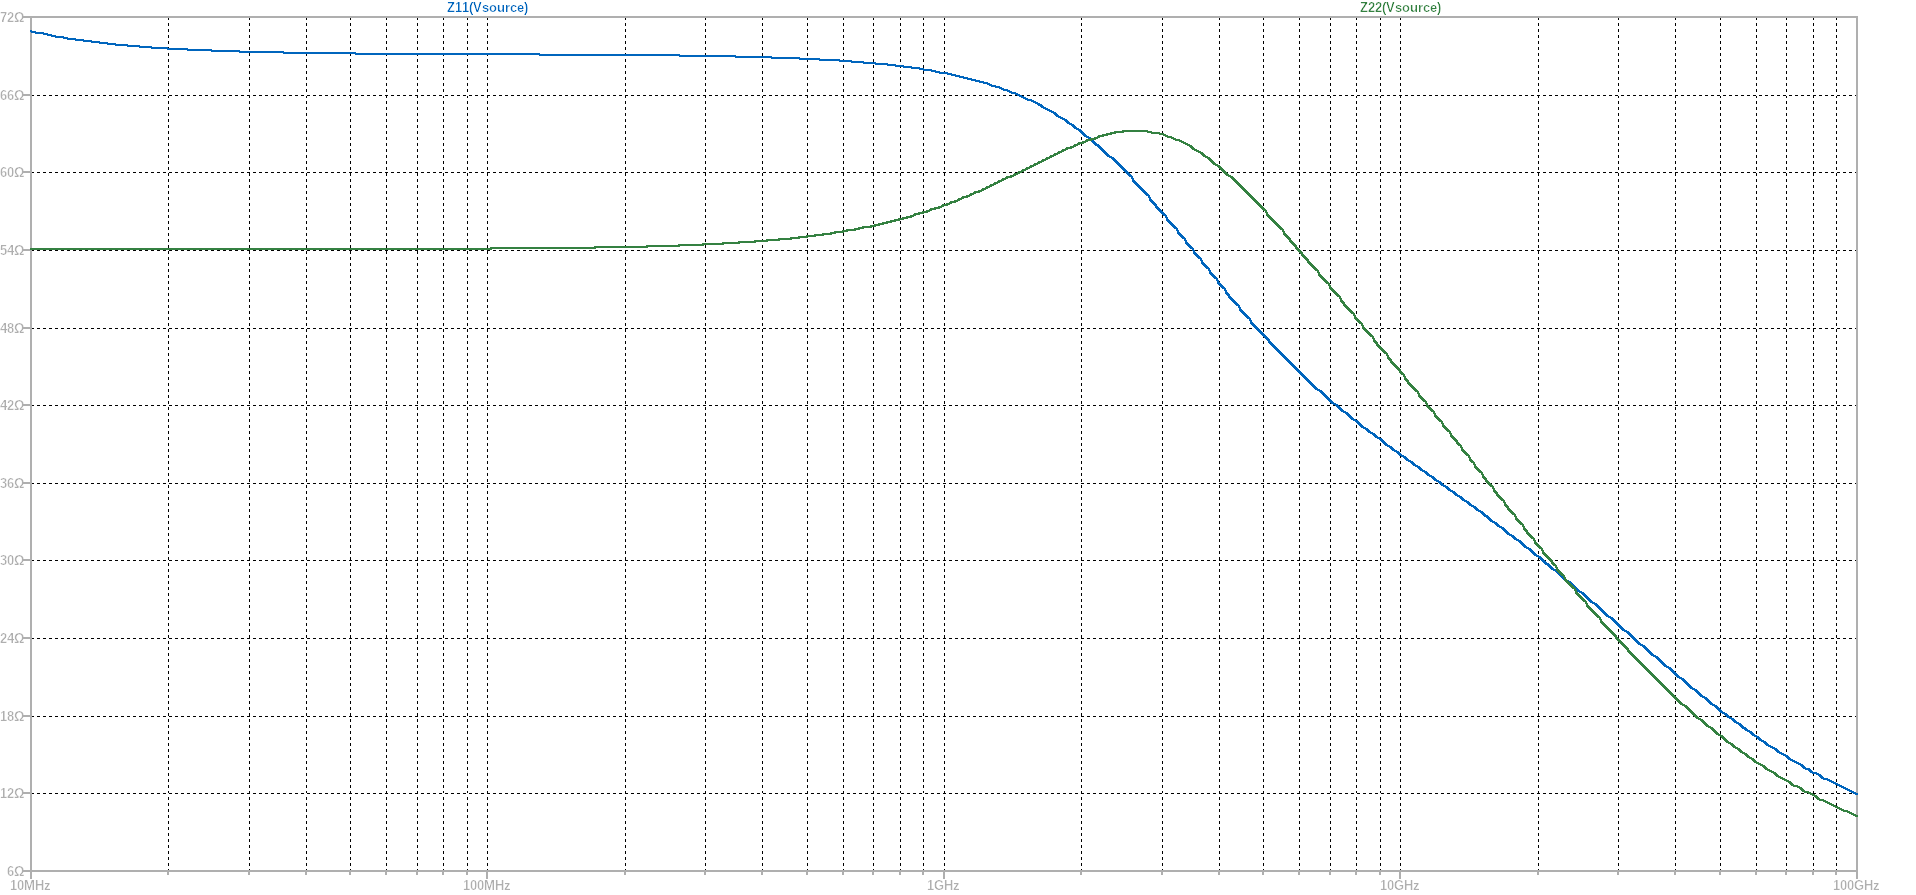
\includegraphics[width=1\textwidth]{Images/Imp_45_1To1.png}
    \caption{Input and Output Impedances for 45 nm Technology with 1:1 $g_m$ Ratio}
    \label{fig:ZParam45nm1to1}
\end{figure}

Lastly the simulation of the noise factor is shown in Figure \ref{fig:Noise45nm1to1}.
\begin{figure}[H]
    \centering
    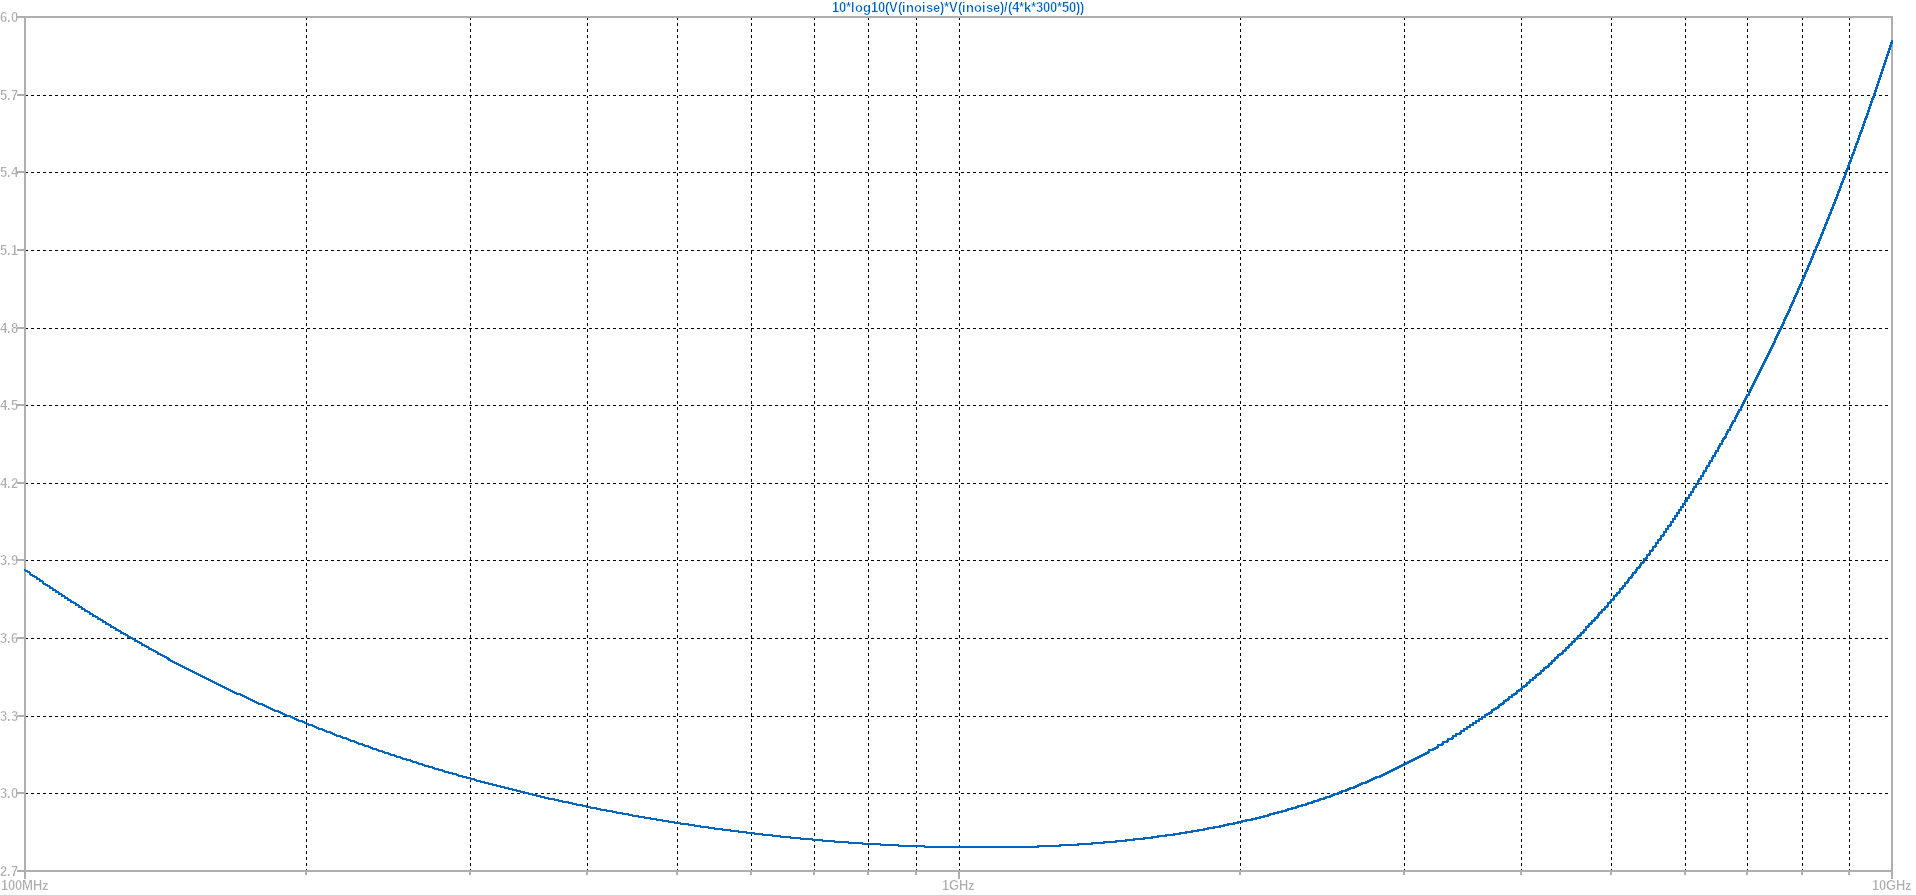
\includegraphics[width=1\textwidth]{Images/Noise_45_1To1.png}
    \caption{Noise Figure for 45 nm Technology with 1:1 $g_m$ Ratio}
    \label{fig:Noise45nm1to1}
\end{figure}

\begin{table}[H]
    \centering
    \caption{Simulation Results for 45 nm Technology with 1:1 $g_m$ Ratio}
    \begin{tabularx}{\textwidth}{>{\centering\arraybackslash}X >{\centering\arraybackslash}X }
        \toprule
        \textbf{Parameter} & \textbf{Value}\\
        \midrule
        Gain (S21) & \SI{4.84}{\decibel} \\
        \midrule
        Noise Figure (NF) & \SI{3.76}{\decibel} \\
        \midrule
        Input Impedance (Z11) & \SI{57}{\ohm} \\
        \midrule
        Output Impedance (Z22) & \SI{47.5}{\ohm} \\
        \midrule
        Frequency & \SI{5}{\giga \hertz} \\
        \bottomrule
    \end{tabularx}
    \label{tab:45nm_1to1_results}
\end{table}
\subsubsection{1:3 $g_m$ ratio}

The results of the s parameters for the 45 nm technology with a 1:3 $g_m$ ratio are shown in Figure \ref{fig:SParam45nm1to3}. 
\begin{figure}[H]
    \centering
    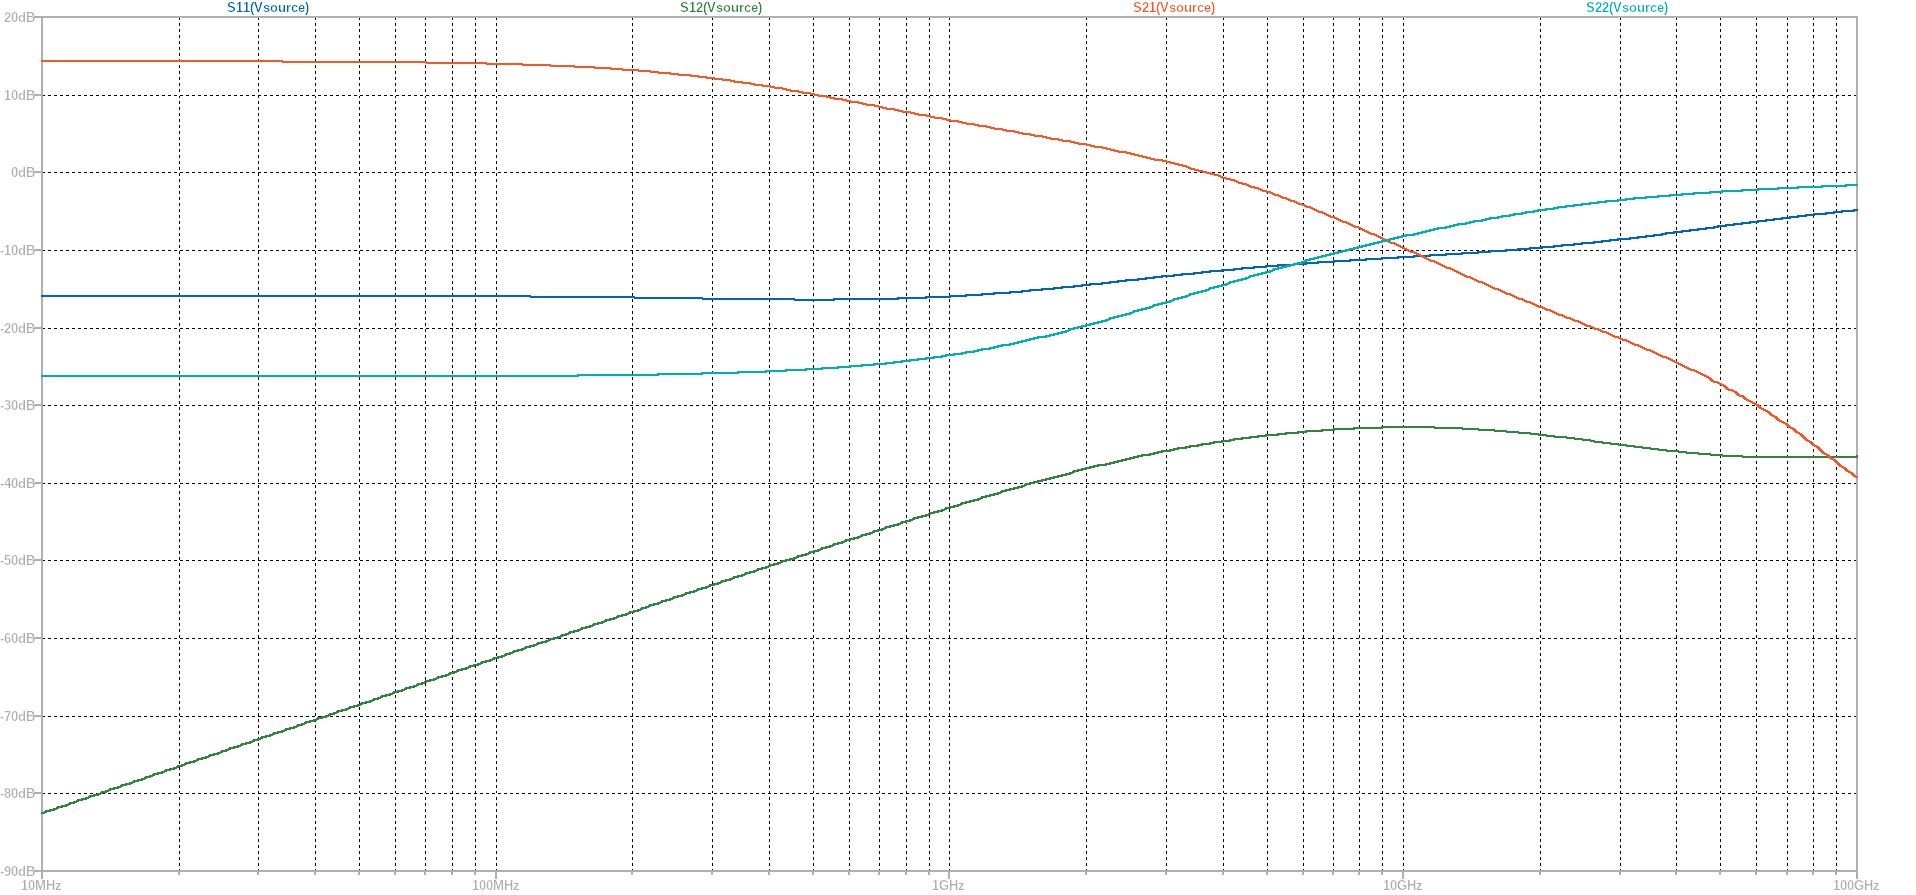
\includegraphics[width=1\textwidth]{Images/SParam_45_1To3.png}
    \caption{S parameters simulation for 45 nm Technology with 1:3 $g_m$ Ratio}
    \label{fig:SParam45nm1to3}
\end{figure}

The results for the input and output impedances are shown in Figure \ref{fig:ZParam45nm1to3}.

\begin{figure}[H]
    \centering
    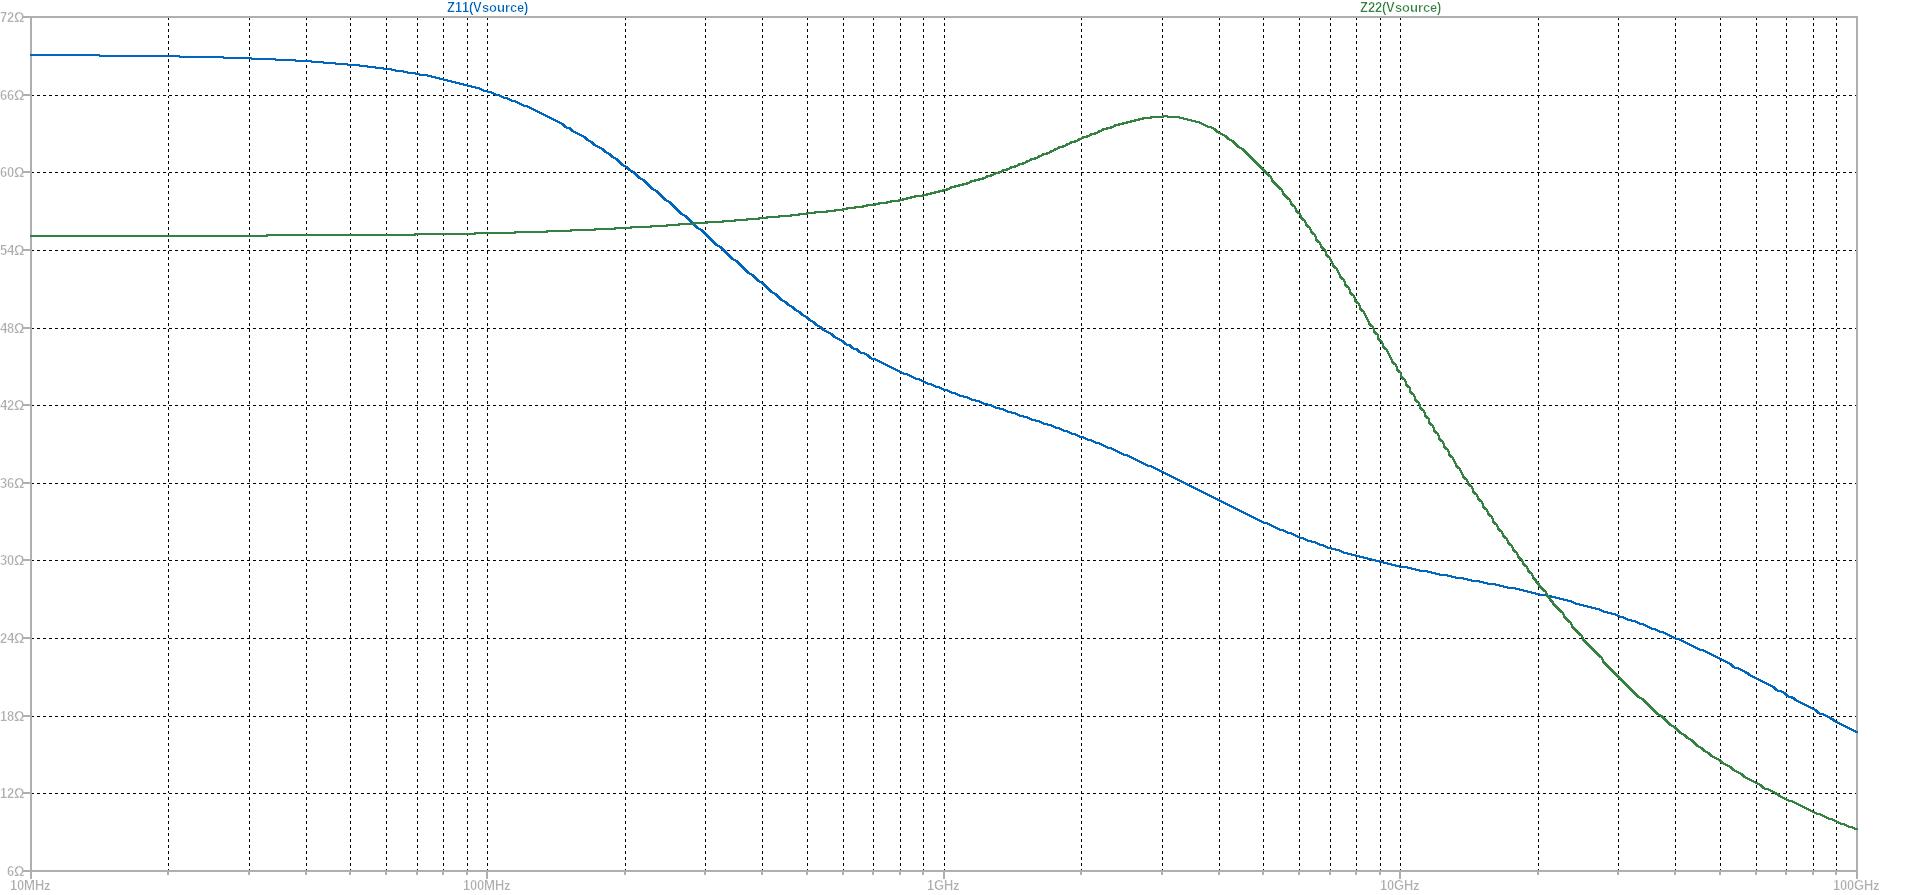
\includegraphics[width=1\textwidth]{Images/Imp_45_1To3.png}
    \caption{Input and Output Impedances for 45 nm Technology with 1:3 $g_m$ Ratio}
    \label{fig:ZParam45nm1to3}
\end{figure}

Lastly the simulation of the noise factor is shown in Figure \ref{fig:Noise45nm1to3}.
\begin{figure}[H]
    \centering
    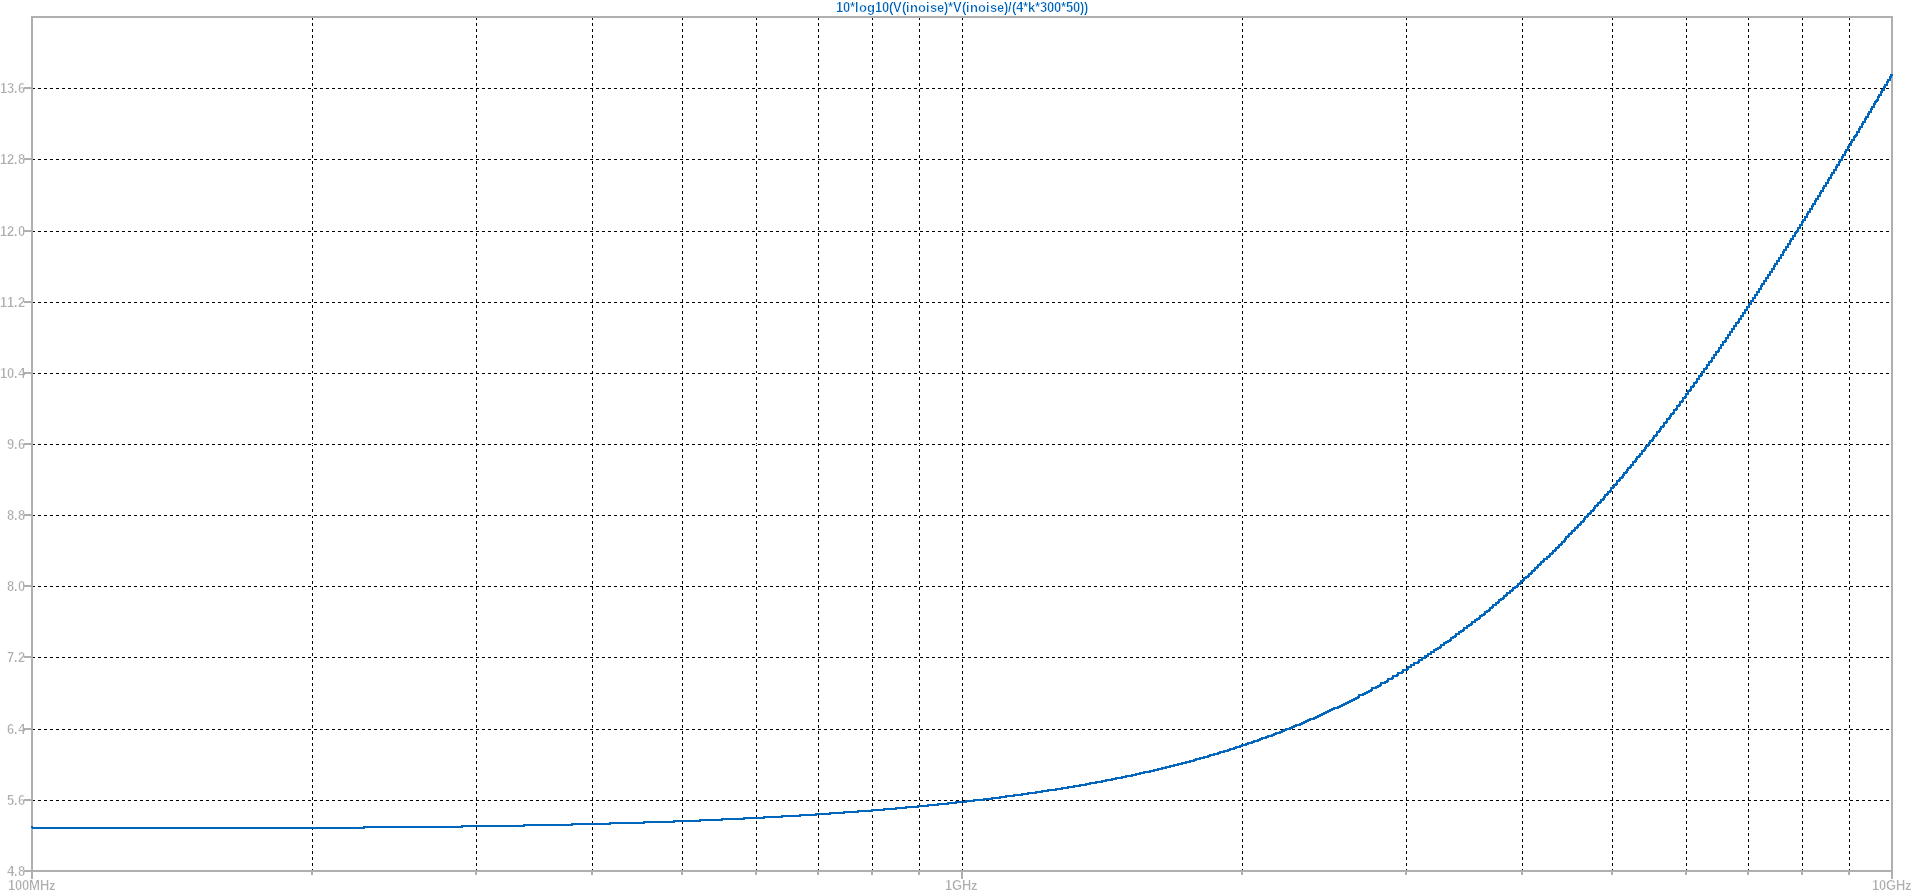
\includegraphics[width=1\textwidth]{Images/Noise_45_1To3.png}
    \caption{Noise Figure for 45 nm Technology with 1:3 $g_m$ Ratio}
    \label{fig:Noise45nm1to3}
\end{figure}

\begin{table}[H]
    \centering
    \caption{Simulation Results for 45 nm Technology with 1:3 $g_m$ Ratio}
    \begin{tabularx}{\textwidth}{>{\centering\arraybackslash}X >{\centering\arraybackslash}X }
        \toprule
        \textbf{Parameter} & \textbf{Value}\\
        \midrule
        Gain (S21) & \SI{1.4}{\decibel} \\
        \midrule
        Noise Figure (NF) & \SI{7}{\decibel} \\
        \midrule
        Input Impedance (Z11) & \SI{36}{\ohm} \\
        \midrule
        Output Impedance (Z22) & \SI{64}{\ohm} \\
        \midrule
        Frequency & \SI{3}{\giga \hertz} \\
        \bottomrule
    \end{tabularx}
    \label{tab:45nm_1ton_results}
\end{table}

\subsection{Results Analysis and Technology Nodes Comparison}

Table~\ref{tab:summary-results} summarizes the key performance metrics obtained from simulations across different CMOS technology nodes and $g_m$ ratios. The results reveal clear trends in how technology scaling affects gain, noise figure (NF), and impedance matching, as well as the limitations introduced by advanced process nodes.

The 45~nm node presented the weakest performance. In both $1{:}1$ and $1{:}3$ configurations, the gain fell well below the 10~dB target, and the NF exceeded the maximum 3~dB specification. These shortcomings stem from increased parasitic capacitances, lower intrinsic gain, and reduced voltage headroom. Additionally, short-channel effects and early high-frequency poles degraded impedance flatness and linearity. These factors render the 45~nm node unsuitable for this LNA design.

In contrast, the 350~nm technology node achieved solid performance. Both configurations surpassed the gain requirement, and the $1{:}3$ configuration also succeeded in reducing the noise figure to 2.64~dB. Although the input impedance dropped slightly to 45.58~$\Omega$, this is still acceptable. These results are consistent with expectations for older CMOS nodes, where longer channels provide higher output resistance and reduced variability, at the cost of increased area and power consumption.

The 65~nm node emerged as the optimal choice. The $1{:}1$ configuration showed excellent gain (10.94~dB) but slightly exceeded the NF limit (3.29~dB). However, the $1{:}n$ configuration fully met all specifications, achieving 10.86~dB gain and 2.49~dB NF, with input/output impedances close to the \SI{50}{\ohm} target. This reflects the ideal trade-off of moderate technology scaling, this is,  reduced parasitics and sufficient headroom to maintain analog performance, while enabling dense integration.

From a broader perspective, these results reinforce the advantages of intermediate CMOS nodes like 65~nm, where analog performance remains robust and compatible with advanced digital integration. While older nodes like 350~nm resemble the behavior of bipolar devices—providing strong gain and linearity—they are less scalable and efficient. On the other hand, deeply scaled technologies like 45~nm, although optimal for high-speed logic, present considerable challenges for analog design due to aggressive short-channel effects.

\begin{table}[H]
    \centering
    \caption{Summary of LNA Simulation Results}
    \begin{tabularx}{\textwidth}{
        >{\centering\arraybackslash}X
        >{\centering\arraybackslash}X
        >{\centering\arraybackslash}X
        >{\centering\arraybackslash}X
        >{\centering\arraybackslash}X
        >{\centering\arraybackslash}X
        >{\centering\arraybackslash}X
    }
        \toprule
        Tech Node & $g_m$ Ratio & Gain (dB) & NF (dB) & $Z_{in}$ ($\Omega$) & $Z_{out}$ ($\Omega$) & Meets Specs \\
        \midrule
        350 nm & 1:1 & 10.52 & 3.19 & 50.84 & 57.94 & Partial \\
        350 nm & 1:3 & 10.58 & 2.64 & 45.58 & 56.82 & Yes \\
        65 nm  & 1:1 & 10.94 & 3.29 & 44.68 & 55.49 & No \\
        65 nm  & 1:n & 10.86 & 2.49 & 56.68 & 44.95 & Yes \\
        45 nm  & 1:1 & 4.84  & 3.76 & 57.00 & 47.50 & No \\
        45 nm  & 1:3 & 1.40  & 7.00 & 36.00 & 64.00 & No \\
        \bottomrule
    \end{tabularx}
    \label{tab:summary-results}
\end{table}
